\documentclass{report}
\usepackage[a4paper, portrait, top=20mm, left=20mm, right=20mm, bottom=20mm]{geometry}
\usepackage{graphicx,wrapfig,amsmath,amssymb,xcolor,pgfplots,adjustbox,float,amsthm,mdframed,subcaption,bm,euler,physics,amsfonts}
\usepackage[colorlinks=true,urlcolor=blue]{hyperref}
\usepackage[linesnumbered,ruled,vlined]{algorithm2e}
\usepackage[utf8]{inputenc}

\newtheorem{theorem}{Theorem}[section]
\newtheorem{corollary}{Corollary}[theorem]
\newtheorem{lemma}[theorem]{Lemma}
\newtheorem*{solution}{Solution}

\newcommand{\w}{\mathbf{w}} % vectors
\newcommand{\x}{\mathbf{x}}
\newcommand{\y}{\mathbf{y}}
\newcommand{\X}{\mathbf{X}}
\newcommand{\Y}{\mathbf{Y}}
\newcommand{\Pb}{\mathcal{P}}
\newcommand{\D}{\mathcal{D}}
\newcommand{\Beta}{\mathcal{B}}
\newcommand{\where}{\textrm{ where }}
\newcommand{\hxt}{h\left(\widetilde{\x}\right)}
\newcommand{\xt}{\tilde{x}}
\newcommand{\yt}{\tilde{y}}
\newcommand{\expe}[1]{\mathbb{E}\left[#1\right]}
\newcommand{\tc}{\textbf}
\newcommand{\pipe}{\ | \ }

\DeclareMathOperator*{\argmax}{arg\,max}
\DeclareMathOperator*{\argmin}{arg\,min}

\newcommand{\loss}{\mathcal{L}}

\setlength{\parindent}{0pt}

\title{Artificial Intelligence and Machine Learning}
\author{Abhijit Amrendra Kumar}
\date{August 2023}

\begin{document}
\maketitle

\chapter{Introduction}
\section{What is Machine Learning ?}

Machine learning is the ability of machines to \tc{learn} from data or past experiences, which come from various sources such as sensors, domain knowledge, experimental runs, etc. Mathematically, it involves making a theoretical function/model $f: X \rightarrow Y$ which predicts outcomes from given inputs, and optimizing it and training it to increase it's prediction accuracy.

\section{Why Machine Learning ?}

We need machine learning in the following cases
\begin{itemize}
  \item When we need to perform tasks that are easy for humans, but complex for computer systems to emulate (eg. distinguishing between a muffin and a Chihuahua)
  \item When we need to perform tasks which are beyond human capabilities, like the analysis of large and complex datasets
\end{itemize}

\begin{center}
  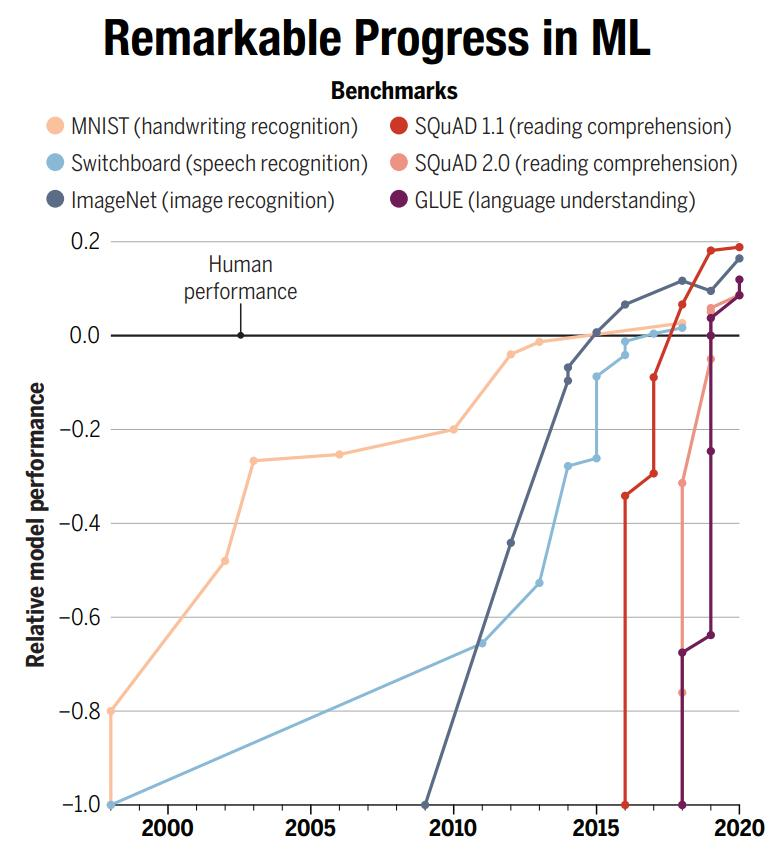
\includegraphics[scale=0.25]{"images/01.jpg"}
\end{center}

Here is a usage histogram for various ML algorithms, which indicates that linear regression and decision trees are very likely to be useful in a machine learning problem.

\begin{center}
  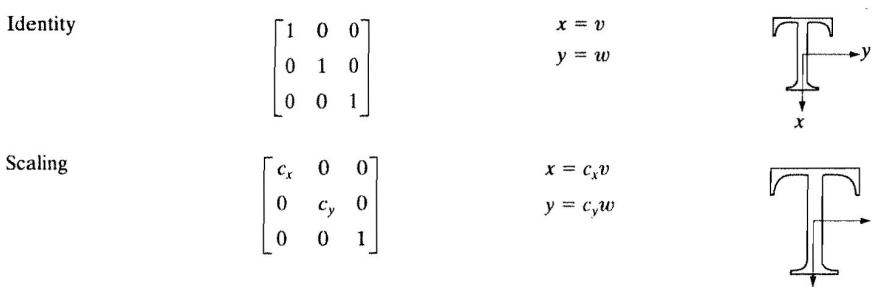
\includegraphics[scale=0.2]{"images/02.png"}
\end{center}

\section{ML Pipeline}
\begin{itemize}
  \item \tc{Data}: Collect data for your problem
        \begin{itemize}
          \item Is the data labelled or unlabelled ?
        \end{itemize}
  \item \tc{Representation}: Choose features that represent your data
        \begin{itemize}
          \item Is the data representation raw, expert-derived or learned ?
        \end{itemize}
  \item \tc{Modeling}: Choose a model for a task
        \begin{itemize}
          \item Should the model be linear/non-linear ? Also, what will be the computational overheads ?
        \end{itemize}
  \item \tc{Training/Learning}: Model will (likely) be parameterized, and these parameters will be learned by training over the data. So, choose a loss function to optimize.
        \begin{itemize}
          \item Which loss function to choose ? And how to best optimise this loss function ?
        \end{itemize}
  \item \tc{Prediction/Inference}: Given a model, assign labels to unseen test instances, then choose an evaluation metric.
        \begin{itemize}
          \item Is the evaluation manual or automatic ?
        \end{itemize}
\end{itemize}

\section{Resources}
Here are some links to find various datasets
\begin{itemize}
  \item \href{https://archive.ics.uci.edu/}{https://archive.ics.uci.edu/}
  \item \href{https://huggingface.co/datasets}{https://huggingface.co/datasets}
  \item \href{http://www.openslr.org/}{http://www.openslr.org/}
\end{itemize}
\chapter{Linear Regression}

\section{Notation}

In general we format variables as: $x$ for scalars, $\x$ for vectors, and $X$ for matrices.
\begin{itemize}
  \item Input / Feature space / Attributes Space :  \(\mathcal{X} =  \mathbb{R}^d\) for some \(d\in\mathbb{N}\)
  \item Output / \emph{Label space} / Response space : \( \mathcal{Y}= \mathbb{R} \)
  \item Dataset : \( \D = \left\{(\tc{x}_i,y_i)\right\}_{i=1}^{n} \), where \(\tc{x}_i \in \mathcal{X}, y_i \in \mathcal{Y} \ \forall \ i \in \{1\ldots n\}\)
\end{itemize}

We consider a target function $f : \mathcal{X} \to \mathcal{Y}$ on the training dataset $\D$, i.e. $\tc{x} \overset{f}{\mapsto} y \ \forall \ (\x,y) \in \D$. \\

We focus on the task of finding a \emph{hypothesis function} \(h : \mathcal{X} \to \mathcal{Y}\) that ideally closely approximates \(f\). We call the family of the hypothesis functions as \(\mathcal{H}\), the \emph{Hypothesis Class}. It follows that \(h \in \mathcal{H}\)
This now brings the following questions:
\begin{enumerate}
  \item What are the possibilities for the predictor function \(h\) ? [\tc{Hypothesis Class}]
  \item How do you quantify the performance of the predictor? [\tc{Loss/Error Function}]
  \item How do we find the best predictor? [\tc{Optimization}]
\end{enumerate}

\section{What are the possible predictor functions?}

Let us first play with a simpler case with a one-dimensional feature space. We may consider the problem as a line fitting problem, taking our hypothesis class to be all linear functions.

\begin{figure}[H]
  \centering
  \begin{tikzpicture}
    \begin{axis}[
        axis lines=middle,
        xlabel=$x$,
        ylabel=$y$,
        xmin=0, xmax=10,
        ymin=0, ymax=15,
        xtick={0,2,...,5},
        ytick={0,3,...,9},
        grid=both,
        grid style={line width=0.1pt, draw=gray!30},
      ]
      \addplot[only marks, mark=*, blue] coordinates {
          (1, 2)
          (2, 4)
          (3, 5)
          (4, 7)
          (5, 8)
          (2,9)
          (4,2)
          % Add more data points here
        };
      \addplot[red] {1.5*x + 0.5}; % Change the slope and intercept as needed
    \end{axis}
  \end{tikzpicture}
  \caption{Fitting a line to the data}
\end{figure}

Let us parametrize the line with $w_0,w_1$ (intercept and slope). We can vectorize our parameters as $W = \begin{bmatrix} w_0 \\ w_1 \end{bmatrix}$. Then we may write our hypothesis function $h_\w$ parametrised by $\w$ as.

$$
  h_\w(x) = w_0 + w_1 x
$$

Let us also vectorize our input as $\x = \begin{bmatrix} 1 \\ x \end{bmatrix}$, so that
$$
  h_{\w}(\x) = \tr{\w} \x
$$

We can now extend this to the multidimensional case. We consider our function to return a linear combination of our \(d\) dimensional features. \newline

\begin{figure} [h]
  \centering
  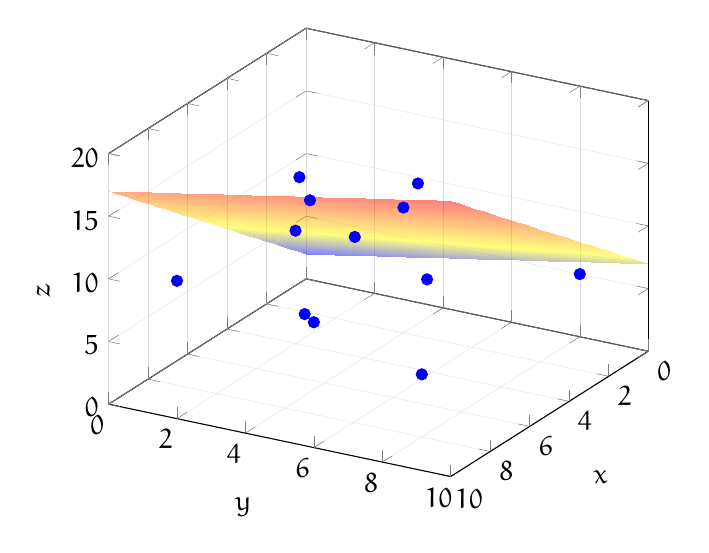
\begin{tikzpicture}
    \begin{axis}[
        view={120}{30},
        xlabel=$x$,
        ylabel=$y$,
        zlabel=$z$,
        xmin=0, xmax=10,
        ymin=0, ymax=10,
        zmin=0, zmax=20,
        xtick={0,2,...,10},
        ytick={0,2,...,10},
        ztick={0,5,...,20},
        grid=both,
        grid style={line width=0.1pt, draw=gray!30},
      ]

      \addplot3[only marks, mark=*, blue] coordinates {
          (0,8,5)
          (1, 2, 5.5)
          (2, 4, 10)
          (3, 5, 13.5)
          (4, 2, 9)
          (5, 3, 13)
          (6, 7, 10)
          (7, 4, 6.5)
          (8, 8, 5)
          (9, 5, 20)
          (10, 6, 10)
          (10, 2, 11)
        };

      \addplot3[
        surf,
        opacity=0.5,
        shader=interp,
        domain=0:10,
        domain y=0:10,
      ] {1.5*x + 0.5*y + 2}; % Adjust the coefficients as needed

    \end{axis}
  \end{tikzpicture}
  \caption{For higher dimensional feature spaces, linear regression is akin to \emph{Hyperplane Fitting}}
\end{figure}

We now have our parameter \(\w = \begin{bmatrix}w_0\\w_1\\\vdots\\w_d\end{bmatrix} \in \mathbb{R}^{d+1}\) and input vector \(\x = \begin{bmatrix}1\\x_1\\\vdots\\x_d\end{bmatrix}\) to get a identical expression -

$$
  h_\w(\x) = \tr{\w} \x
$$
Our hypothesis class is, then -
$$
  \mathcal{H} = \{ h_\w : \w \in \mathbb{R}^{d+1} \}
$$

This is essentially the \textit{linear} in linear regression. However, note that it does not mean we are restricted to linear functions of the features, we may transform the feature space to another space to regress.

\section{How to quantify the performance of a predictor ?}

We define a function that operates on the predictor function and dataset to quantify the "mismatch" between the two. Higher the loss function, lesser is the given predictor suitable for the dataset. Given that our function is parametrized, we may also define the loss function in terms of the parameter.

$$
  \text{Loss Function: } \loss(h,\D) ~\text{or}~ \loss(\w,\D)
$$

Let us consider a singleton dataset $\D_{test} =\{(\x,y)\}$ where $\x = \tr{\left[1~x_1~\ldots~x_d\right]}$. We define a loss for this dataset as
$$
  \loss(\w,\D_{test}) = (y-h_\w(\x))^2 = |y-\hat{y}|^2
$$

We define \(h_\w(x) = \hat{y}\), and \(|y-\hat{y}|\) is called a \emph{residual}. \\

Now for a dataset containing $n$ datapoints,

$$
  \mathbf{Least\ Squares\ Loss:} \ \  \loss(\w,\D_{train}) = \frac{1}{n} \sum_{i=1}^n(y_i-h_\w(\x_i))^2 = \frac{1}{n} \sum_{i=1}^n \left|y_i - \hat{y}_i\right|^2
$$

Note that the least squares loss is the mean of the squares of the residuals. We can also define a loss equal to the mean residual value.

$$
  \text{Mean Absolute Error Loss:} \ \ \loss({\w,\D_{train}}) = \frac{1}{n} \sum_{i=1}^n \left|y_i - \hat{y}_i\right|
$$

The Mean Absolute Error does not penalise high deviations as much as the Squares Loss, thus it may be more appropriate to use when the dataset contains many outliers.
\begin{figure}[htbp]
  \centering
  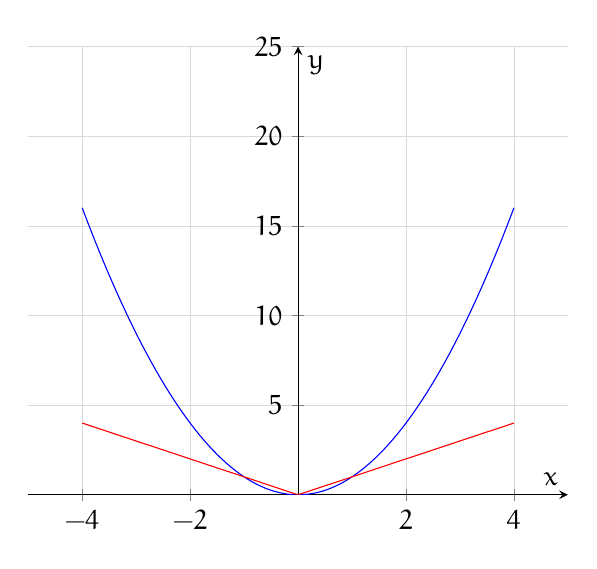
\begin{tikzpicture}
    \begin{axis}[
        axis lines=middle,
        xlabel=$x$,
        ylabel=$y$,
        xmin=-5, xmax=5,
        ymin=0, ymax=25,
        xtick={-4,-2,0,2,4},
        ytick={0,5,10,15,20,25},
        grid=both,
        grid style={line width=0.1pt, draw=gray!30},
      ]
      \addplot[blue, domain=-4:4, samples=100] {x^2};
      \addplot[red, domain=-4:4, samples=100] {abs(x)};
    \end{axis}
  \end{tikzpicture}
\end{figure}

Here we are interested in the least squares loss. We can vectorize the loss function as follows

$$
  \boxed{\mathbf{\loss(\w, \D_{\text{train}}) = \frac{1}{n} \lVert \y \mathrm{-} X\w \rVert_2^2}}
$$

$$
  \text{, where } X =
  \begin{bmatrix}
    \longleftarrow{\tr{\x_1}} \longrightarrow \\
    \longleftarrow \tr{\x_2} \longrightarrow  \\
    \vdots                                    \\
    \longleftarrow \tr{\x_n} \longrightarrow
  \end{bmatrix}_{n\times (d+1)}, \quad
  \y =
  \begin{bmatrix}
    y_1    \\
    y_2    \\
    \vdots \\
    y_n
  \end{bmatrix}_{n\times 1}\quad
$$

\section{How do we find the best predictor?}

We use the loss function to find our optimum hypothesis $h^*$, where
$$
  h^* = \argmin_{h \in \mathcal{H}} \loss(h,\D_{train})
$$

[Note that the optimisation is performed only over the training dataset]

We may also define the objective in terms of the parameter $\w$ corresponding to $h$.

\begin{align*}
  \w^*    & = \argmin_{\w} \loss(\w,\D_{train})            \\
  \w_{LS} & = \argmin_{\w} \sum_{i=1}^n(y_i-\tr{\w} x_i)^2
\end{align*}

We set out to find a closed form solution for \(\w_{LS}\) for $d$ dimensional data:

To find the optimum, we set the derivative\footnotemark[1] to zero. We may drop the \(\frac{1}{n}\) term.
\begin{align*}
  \nabla_\w\loss & = \frac{\partial{\loss(\w,\D_{train})}}{\partial{\w}} = \left[\frac{\partial{\loss(\w,\D_{train})}}{\partial{w_i}}\right]_{i=1}^n = \left[-2(y_i-\tr{\w} x_i)x_i\right]_{i=1}^n = 0 \\
  \implies       & 2(-\tr{X} \y + \tr{X} X\w) =0                                                                                                                                                       \\
  \implies       & \w_{LS} = (\tr{X} X)^{-1}\tr{X} Y
\end{align*}

We can also derive this result with vector-derivative identities\footnotemark[1],
\begin{align*}
           & \nabla_\w\loss = 0                                                                                                                                       \\
  \implies & \frac{\partial }{\partial \w} \lVert \y-X\w\rVert_2^2 = \frac{\partial}{\partial \w}\left(\tr{\y}\y - 2\tr{\w} \tr{X} \y + \tr{\w} \tr{X} X\w\right) = 0 \\
  \implies & -2\tr{X} \y + 2\tr{X}X\w = 0                                                                                                                             \\
  \implies & \tr{X}X\w = \tr{X}\y                                                                                                                                     \\
           & \boxed{\w = (\tr{X} X)^{-1}(\tr{X} \y)}
\end{align*}
Note that \(\tr{X}X\) need not be invertible.

\section{Homework}
For 1D data, $ h_\w(x)=w_0+w_1 x $,
prove that --
\begin{equation*}
  {\w_1}^* = \frac{\sum (x_i-\bar{x})(y_i-\bar{y})}{\sum (x_i-\bar{x})^2}
\end{equation*}

where \(\bar{x} = \frac{\sum{x_i}}{N} \text{ \ and \ } \bar{y} = \frac{\sum{y_i}}{N}\).

\begin{solution}
  \begin{align*}
    \mathcal{L}                               & = \sum_{i=1}^N (y_i-w_0-w_1x_i)^2                                                     \\
    \frac{\partial \mathcal{L}}{\partial w_0} & = - \sum_{i=1}^N (y_i-w_0-w_1x_i) = 0                                                 \\
    \implies  w_0^*                           & = \bar{y} - w_1\bar{x}                                                                \\
    \frac{\partial \mathcal{L}}{\partial w_1} & = - \sum_{i=1}^N x_i(y_i-w_0-w_1x_i) = 0                                              \\
    \implies w_1^*                            & = \frac{\sum_{i=1}^N x_iy_i - Nw_0^*\bar{x}} {\sum_{i=1}^N x_i^2}                     \\
                                              & = \frac{\sum_{i=1}^N x_iy_i - N\bar{x}\bar{y} + w_1^*N\bar{x}^2} {\sum_{i=1}^N x_i^2} \\
                                              & = \frac{\sum_{i=1}^N (x_iy_i - \bar{x}\bar{y})} {\sum_{i=1}^N (x_i-\bar{x})^2}        \\
                                              & = \frac{\sum_{i=1}^N (x_i-\bar{x})(y_i-\bar{y})} {\sum_{i=1}^N (x_i-\bar{x})^2}
  \end{align*}
\end{solution}

\footnotetext[1]{There are two conventions for the derivative of a scalar by a vector, i.e., whether the result is a \href{https://www.cs.huji.ac.il/w~csip/tirgul3_derivatives.pdf}{row} or \href{https://onlinelibrary.wiley.com/doi/pdf/10.1002/0471705195.app3}{column}. Here we will stick with the latter.}

\newpage
\section{Basis Functions}

\begin{center}
  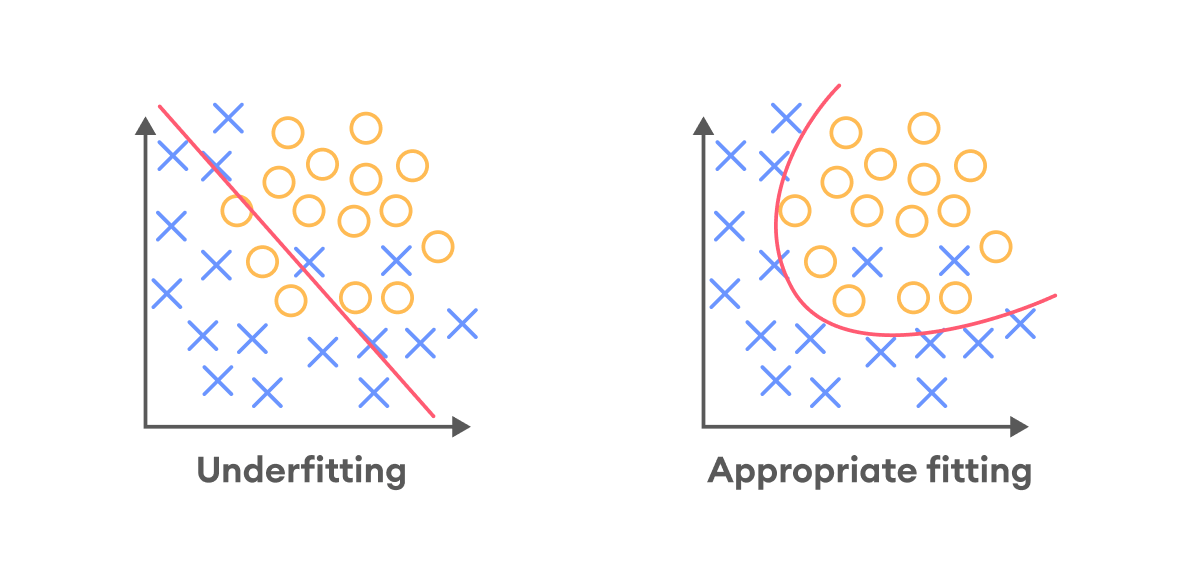
\includegraphics[scale=0.25]{images/03.png}
\end{center}

\begin{itemize}
  \item In the above figure, the left-side model represent  \( h_\w(x) = w_0 + w_1x \) for some \(w_0, w_1\), but it doesn't fit the given dataset well.
  \item Right-side model fits the dataset well, and represents \( h_\w(x) = w_0 + w_1x + w_2x^2 \) for some \(w_0, w_1, w2\).
  \item This suggests we may want to change/transform the feature space we are working with for improved model fits. We detail the procedure below using basis functions.
\end{itemize}

Given a basis function $\phi:\mathcal{X}\rightarrow \mathbb{R}^{m + 1}$, where
\begin{align*}
  \phi(\x) =
  \begin{bmatrix}
    1          \\
    \phi_1(\x) \\
    \phi_2(\x) \\
    \vdots     \\
    \phi_m(\x)
  \end{bmatrix}_{(m + 1)\times 1}
\end{align*}
The hypothesis space becomes
\begin{align*}
  \mathcal{H}_\phi = \left\{\left.h_\mathbf{w} \in \mathcal{X}^\mathbb{R}\right|\mathbf{w}\in\mathbb{R}^{m + 1}, h_\mathbf{w}(\x) = \mathbf{w}^\top\phi(\x)\text{ for }\x \in \mathcal{X}\right\}
\end{align*}

The design matrix with basis function-based transformations can be written as:
\begin{align*}
  \mathbf{\Phi}_\D =
  \begin{bmatrix}
    \phi(\x_1)^\top \\
    \phi(\x_2)^\top \\
    \vdots          \\
    \phi(\x_n)^\top
  \end{bmatrix}_{n\times(m + 1)}
\end{align*}
Note that $\mathbf{\Phi}_\D$ yields $m$-dimensional feature vectors, that could be smaller or larger than the original $d$-dimensional input feature space.

The least-squares objective using basis functions can be written as:
\begin{align*}
  \mathcal{L}_{\text{LS}}(h_\mathbf{w}, \D) & = \dfrac{1}{n}\sum_{i = 1}^n(y_i - h_\mathbf{w}(\x_i))^2           \\
                                            & = \dfrac{1}{n}\sum_{i = 1}^n(y_i - \mathbf{w}^\top\phi(\x_i))^2    \\
                                            & = \dfrac{1}{n}\norm{ \mathbf{y} - \mathbf{\Phi}_\D\mathbf{w} }_2^2
\end{align*}

and as before
\begin{align*}
  \mathbf{w}^*_{\text{LS}} = \left(\mathbf{\Phi}_\D^\top\mathbf{\Phi}_\D\right)^{-1}\mathbf{\Phi}_\D^\top\mathbf{y}
\end{align*}

\newpage
\subsection{Examples of Basis Functions}
\begin{itemize}
  \item \tc{Polynomial Basis}\\ For 1-D data, \(\Phi_j(x) = x^j\) for \(1 \leq j \leq d\) .
  \item \tc{Radial Basis Function(RBF)}\\
        For $d$-dimensional data, \(\Phi_j(\mathbf{x}) = e^{-\frac{\|\mathbf{x}-\mu_j\|_2^2}{\sigma_j^2}}\) for \(\mathbf{x},\mu_j \in \mathbb{R}^d, \sigma_j \in \mathbb{R}\) .
  \item \tc{Fourier Basis}
  \item \tc{Piecewise Linear Basis}
  \item \tc{Periodic Basis ($\sin(x)$, $\cos(x)$ etc.)}
\end{itemize}

\begin{mdframed}
  \tc{Data Splits (Preliminaries)} :
  The original data in a machine learning model is typically taken and split into three sets.
  \begin{itemize}
    \item Training data (Training set): Dataset used to train the model and learn the parameters. (Below, $n$ is the number of data points in the training set)
          \begin{center}$D = \{(\x_i, y_i)\}_{i=1}^n$\end{center}
          \begin{center}Training Error : $\dfrac{\Sigma_{i=1}^n (y_i - h_\w(\x_i))^2}{n}$\end{center}
    \item Development Set (Validation Set) : Mainly used to tune \textit{hyperparameters} of the model. Hyperparameters are not learnable parameters, and are instead predetermined quantities that are used with the model. For example, $\sigma$ in an RBF basis function is a hyperparameter.
    \item Test Set (Evaluation Set) : This is the unseen/test set used for a final evaluation of the model, after choosing the best hyperparameters determined via tuning on the development set. The error on the test set is also referred to as the generalization error.
  \end{itemize}
  Errors on the development/test sets are a measure of the generalization ability of the trained machine learning model.
\end{mdframed}

\section{Hyperparameter tuning}

Hyperparameter tuning involves two general methods :
\begin{itemize}
  \item Grid Search: Define a search space as a grid of hyperparameter values and evaluate every position in the grid.
  \item Random Search: Define a search space as a bounded domain of hyperparameter values and randomly sample points in that domain.
\end{itemize}

\subsection{Underfitting}
Underfitting is a scenario where a data model is overly simple and unable to capture the relationship between the input and output variables accurately.

\begin{figure}[H]
  \centering
  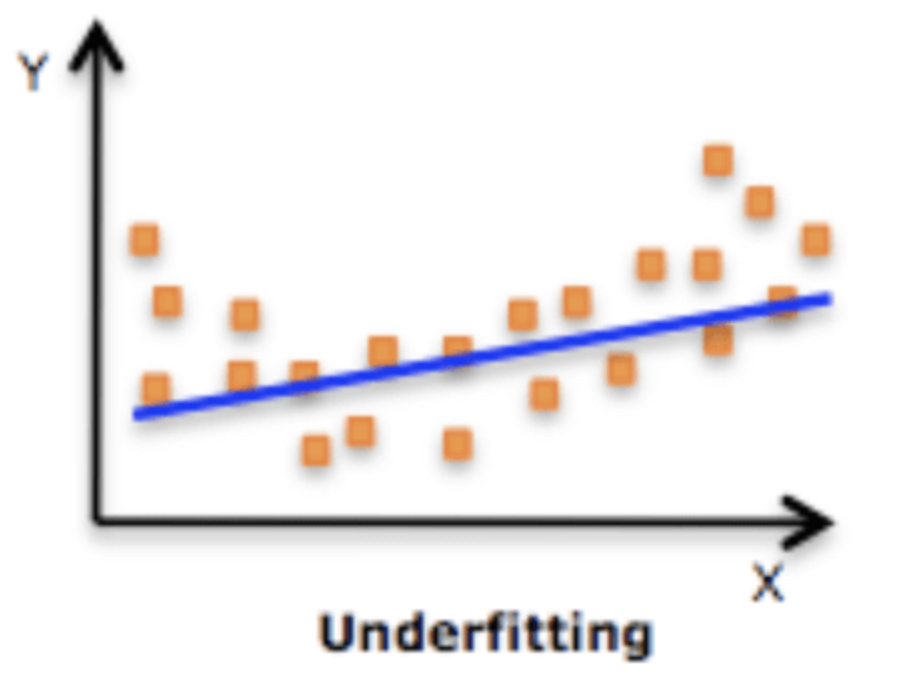
\includegraphics[scale=0.35]{images/04.png}
  \caption{Model is too simple and underfits the data}
\end{figure}

\subsection{Overfitting}
Overfitting is an undesirable machine learning behavior that occurs when the machine learning model gives accurate predictions for training data but not for new data (i.e., does not generalise well). Model fits the training data perfectly but is overly complex.

\begin{figure}
  \begin{subfigure}{0.45\textwidth}
    \centering
    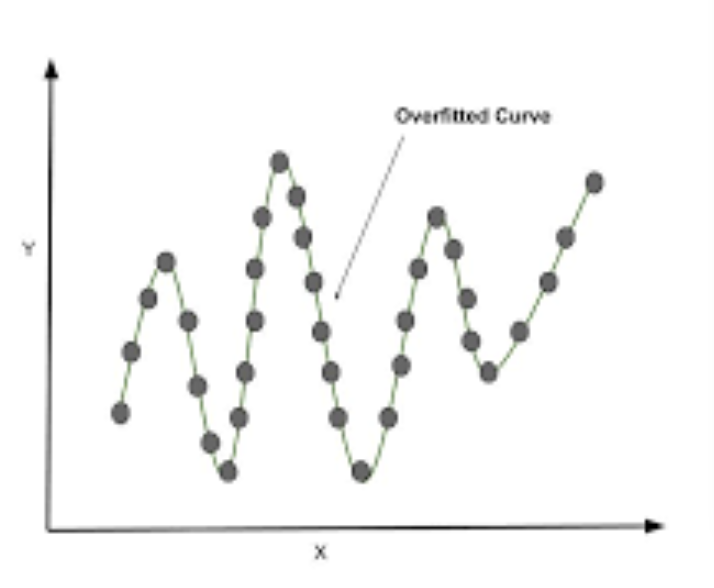
\includegraphics[scale=0.4]{images/05.png}
    \caption{Model is overly complex}
  \end{subfigure}
  \begin{subfigure}{0.45\textwidth}
    \centering
    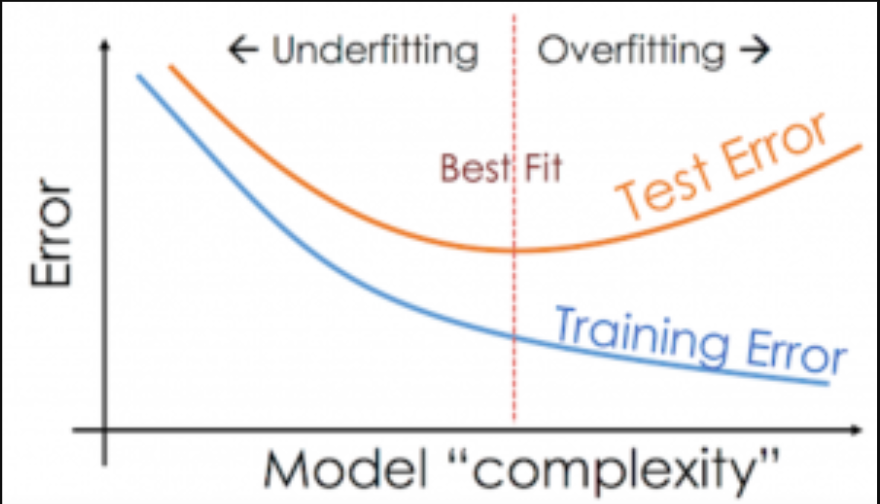
\includegraphics[scale=0.4]{images/06.png}
    \caption{Hyperparameter tuning}
  \end{subfigure}
\end{figure}

It is tempting to assume that having large number of parameters (making complex model) in our hypothesis class would fit the training data perfectly. But this would fail to predict new unseen data miserably. This is termed \tc{overfitting}.

\begin{figure}[H]
  \begin{subfigure}{0.45\textwidth}
    \centering
    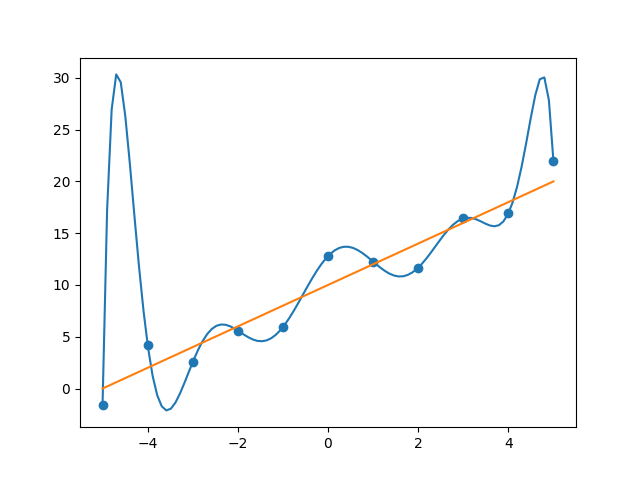
\includegraphics[scale=0.45]{images/07.png}
    \caption{Original}
  \end{subfigure}
  \hfill
  \begin{subfigure}{0.45\textwidth}
    \centering
    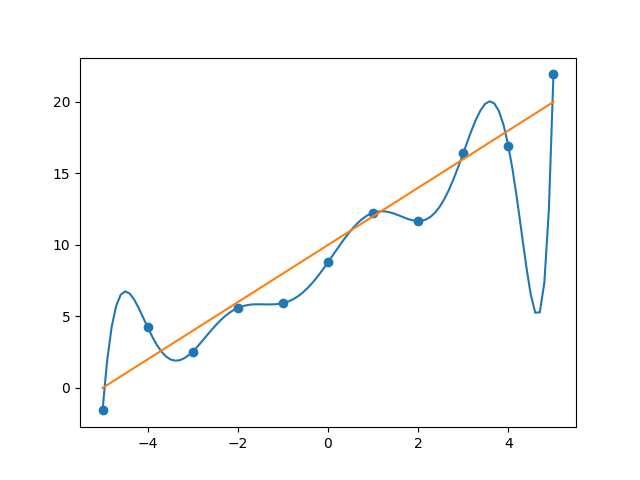
\includegraphics[scale=0.45]{images/08.png}
    \caption{Perturbation}
  \end{subfigure}
  \caption{Overfitting due to complex modelling}
\end{figure}

Consider the line y = 2x+10, let's say we sampled few points from this true line, and this process had some noise involved. In the above figure, we try to fit a polynomial regression model with degree 10. Our predictor function $h_\w(\x)$ is given as:
$$
  h_\w(\x) = w_0 + w_1x + w_2x^2 + \dots + w_{10}x^{10}
$$

It is clearly evident from the image, that the training error is 0, the model perfectly fits the training data, but the test error is fairly high due to the huge variance of the predictor function. Additionally, on small perturbation(here, changing the the data point(0,13) to (0,8) in the second image), has vastly changed the shape of the curve fit, because of several degrees of freedom. \\

Ideally we would want to hit the sweet spot between a simple fit (Underfitting, suffering from high bias) and a complex fit (Overfitting, suffering from high variance), and thus we need to tune the hyperparameter $d$.

\section{Regularization}
Instead of tuning, regularization modifies the loss function to explicitly constrain the model complexity. The general regularised optimisation equation looks like:
$$
  L_{reg}(\w, D_{train}) = L_{MSE}(\w, D_{train}) + \lambda R(\w)
$$

where the first term, $L_{MSE}(\w, D_{train})$ is the measure of fit to the training data set and the second term $\lambda R(\w)$ is the regulariser term, with $\lambda \geq 0$. The $R(\w)$ is a measure of the model's complexity. This can help alleviate overfitting caused by the first term. It does this by penalising/shrinking weights in the weight vector making some of them equal to near zero, Thus even if the model is a high-degree polynomial, minimizing the $L_{reg}$ yields many (near) zero weights, thereby shrinking the model complexity. Two examples of these shrinkage-based regularizations are discussed in the sections below.\\

\fbox{
  \begin{minipage}{\textwidth}
    \tc{Why this works?}
    When the coefficients are very large and the model is highly complex, the errors on dev set or test set are large due to large variances in the predictor function. This can be alleviated by penalising the weight terms(weight norm), thereby making values of $\w$ small, and hence the errors are not every large!
  \end{minipage}
}

\subsection{Ridge Regression}

Ridge regression (also called L2-Normalised Regression) is a regularization technique to combat overfitting. The penalty term $R(\w)$ here is a Euclidean norm, given as $R(\w) = ||\w||^2$. The optimisation objective function and the optimal weights for L2-regularized regression can be written as:
\[ \w_{L_2} = \argmin_\w (||\y-\phi \w||_2^2 + \lambda||\w||_2^2)\]
The above equation is equivalent to the following constrained optimization problem.
\[\w_{L_2} = \argmin_\w ||\y-\phi \w||_2^2 \text{ s.t } ||\w||_2^2 \leq t^2 \]
\fbox{
  \begin{minipage}{\textwidth}
    Note: Usually, we don't include $w_0$ in the penalty term R($\w$). This goes well with the intuition that the intercept doesn't depend on the feature vectors and hence penalising $w_0$ would lead to a poor fit.
  \end{minipage}
}\\

Infact, this optimisation problem has a closed form solution just as the non regularised objective function.
\[\nabla L_{ridge}(\w) = 0\]
\[-2 \phi^T(\y-\phi \w) + 2\lambda \w = 0\]
\[\w_{ridge} = (\phi^T\phi + \lambda I)^{-1} \phi^T\y\]

\fbox{
  \begin{minipage}{\textwidth}
    Note: The best thing about the closed form solution is that such a closed form solution always exists, unlike the unregularized loss function solution, because here the term $\phi^T\phi + \lambda I$ is always invertible(provided the regularization parameter $\lambda > 0$). \\

    A matrix $\X \in \mathbb{R}_{n \times n}$ is positive definite if for any $\tc{v} \neq 0$, $\tc{v}^T\X\tc{v} > 0$. And a positive definite matrix is always invertible. Since $\tc{v}^T\X\tc{v} > 0$ for all $\tc{v} \neq 0$, this implies $\X \tc{v} \neq 0$ for all $\tc{v} \neq 0$, which is the definition of an invertible matrix.\\

    In our case, consider a non zero vector $\tc{v}$,
    $$
      \tc{v}^T(\phi^T\phi + \lambda I) \tc{v} = \tc{v}^T\phi^T\phi \tc{v} + \lambda \tc{v}^T\tc{v} = (\phi \tc{v})^T\phi \tc{v} + \lambda \tc{v}^T \tc{v} = ||\phi \tc{v}||_2^2 + \lambda ||\tc{v}||_2^2
    $$

    The above expression is strictly positive for positive values of $\lambda$.
  \end{minipage}
} \\

\subsection{Lasso Regression}

Also known as L1-normalised regression, Lasso (Least Absolute Shrinkage \& Selection Operation) Regression is a similar technique to Ridge regression, but instead of using Euclidean L2 norm for the penalty, we use the L1 norm. So $R(\w) = ||\w||_1$, and the total loss function can be expressed as:
\begin{equation*}
  \w_{L_1} = \argmin_\w (||\y-\phi \w||_2^2 + \lambda||\w||_1)
\end{equation*}
The equivalent constrained form for the above is:
\begin{equation*}
  \w_{L_1} = \argmin_\w (||\y-\phi \w||_2^2) \text{ s.t } ||\w||_1 \leq t
\end{equation*}
As the L1 norm isn't differentiable, there is no closed form solution for the above optimisation problem. Other methods which can be used to solve for the optimal weights:
\begin{itemize}
  \item Quadratic Programming
  \item Iterative optimisation algorithms (e.g. Gradient Descent)
\end{itemize}

\subsection{Comparison}

L1 Regularization yields sparse weight vectors compared to L2 Regularization. This can be intuitively understood from an example. \\

Referring to the figure below diagram, assume the constrained version of the regularization methods, and the predictor with only two weights $\beta_1$ and $\beta_2$. Say, at $\hat{\beta}$, the MSE is minimised. So around that we draw the contours(ellipses) of the loss function, and the points at which a contour touches the boundary of enclosed area by the constraints (rhombus in Lasso, and circle in Ridge) gives the final optimal weights.\\

There will be a large number of cases, where the contour will touch the square at one of its corners (one weight resulting in zero) as compared to touching the circle on the axes. By extrapolation, we can see that in higher dimensions, the cases where multiple weights are zero will occur much more frequently in Lasso regression due to the sharp boundaries. So Lasso regression will prove to be useful in cases when there are outliers present in the training data and using Ridge regression could result in non-zero weights of undesired features present in the set of basis functions. Lasso can effectively ignore these features by setting their weights to zero. Ridge, with its more gradual constraints, might still assign non-zero weights to these features. \\

\fbox{
  \begin{minipage}{\textwidth}
    \tc{Note}: It is not that always sparsity helps. Infact, for neural networks L2 regularization is most widely used (due to its smoothness). But for many benchmark tasks (feature selection tasks), L1 regularization is preferred and encourages models that utilize a smaller subset of features, which can be valuable for interpretability and reduces computational complexity.
  \end{minipage}
}

\begin{figure}[h]
  \centering
  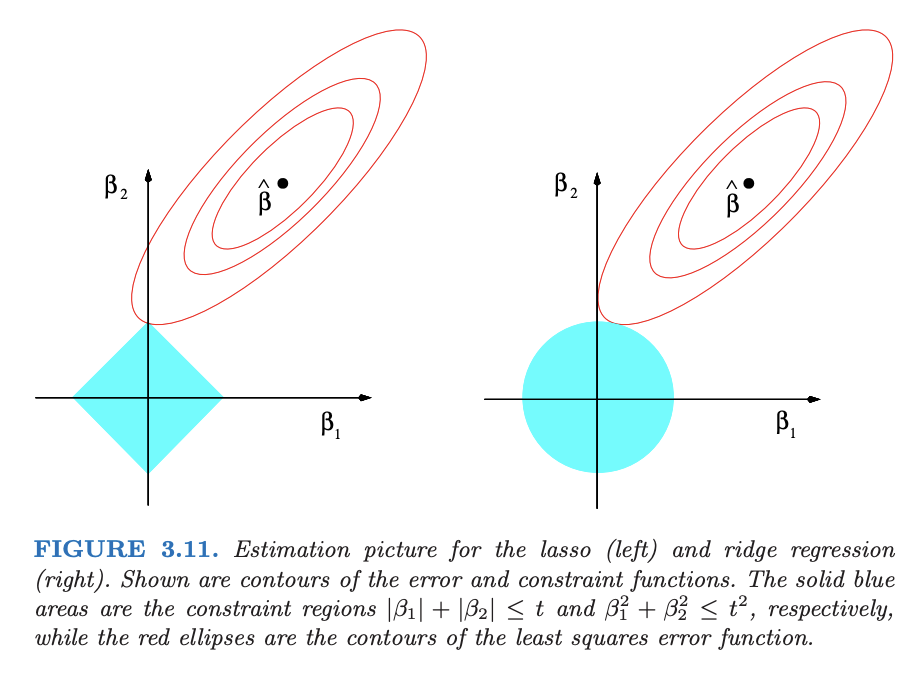
\includegraphics[width=0.7\textwidth]{images/09.png}
  \caption{Comparison of L1 and L2 Regression methods. Figures reproduced from The Elements of Statistical Learning  (Trevor Hastie, Robert Tibshirani and Jerome Friedman. Second Edition. 2009)}
\end{figure}
\chapter{Gradient Descent}

\section{Introduction}
Gradient Descent is a \tc{first-order iterative optimization algorithm} for finding local minimum points of a differentiable function. It's commonly used in machine learning and optimization problems (e.g., matrix factorization, neural networks), especially when dealing with non-convex cost functions that don't have a closed-form solution.
% GD is an iterative optimization algorithm.
\section{General Template of GD-Style Algorithms}
% GD is an iterative optimization algorithm.\\ \\
Let the function being optimized be dependent on the weight vector $\tc{w}$. We now wish to find the optimal value of $\tc{w}$ so that the function in consideration is minimized (since its the loss function which we generally are trying to optimise in ML). GD-style algorithms helps us in finding that. The general flow of such algorithms is as follows:
\begin{itemize}
  \item Initialize {\tc{w}} (e.g. ${\tc{w}} = \Vec{0}$)
  \item Repeat
        \begin{itemize}
          \item Choose a descent direction (directions of fastest decrease)
          \item Choose a step size
          \item Update ${\tc{w}}$
        \end{itemize}
  \item Exit repeat loop when certain stopping criterion is met. Some common stopping criterion include  (where $t$ represents a time step)
        \begin{itemize}
          \item $|| \nabla L(w_{t}) ||_{2} < \epsilon$
          \item $|| {w_{t+1} - w_{t}} ||_{2} < \epsilon$
        \end{itemize}
\end{itemize}
\section{Algorithm of Gradient Descent}
The flow for the Gradient Descent algorithm keeping in the mind the template above is:
\begin{itemize}
  \item $\tc{w} \leftarrow \tc{w}_{0}$ : Initialisation can be done in various ways such as zero initialisation ($w_{0} = \Vec{0}$), randomly sampled Gaussian etc.
  \item For the iterative part, we use the following values :
        \begin{itemize}
          \item Direction : $- \nabla L(\tc{w}_{t})$
          \item Step size (Learning Rate) : $\alpha > 0$ is a hyperparameter
          \item Update : $\tc{w}_{t+1} \leftarrow \tc{w}_{t} - \alpha \nabla L(\tc{w}_{t})$
        \end{itemize}
  \item Some common stopping criteria used among others are:
        \begin{itemize}
          \item $|| \nabla L(w_{t}) ||_{2} < \epsilon$
          \item $|| w_{t+1} - w_{t} ||_{2} < \epsilon$
        \end{itemize}
\end{itemize}

\begin{algorithm}[H]
  \caption{Gradient Descent Algorithm with Epochs}
  \label{algo:gradient_descent_epochs}
  \SetKwInOut{Input}{Input}
  \SetKwInOut{Output}{Output}
  \Input{Initial weight vector $w_0$, step size $\alpha > 0$, tolerance $\epsilon > 0$, maximum number of epochs $N_{\text{max}}$}
  \Output{Optimal weight vector $w^*$}
  $w \gets w_0$\;
  \For{$t \gets 1$ \KwTo $N_{\text{max}}$}{
  Compute gradient direction: $\nabla L(w)$\;
  Update: $w \gets w - \alpha \nabla L(w)$\;
  \If{$||\nabla L(w)||_{2}^{2} \leq \epsilon$}{
  \tc{break}\;
  }
  }
  \Return{$w^* = w$}
\end{algorithm}

\subsection{Why the name Gradient Descent ?}
The name Gradient Descent is made of two parts:
\begin{itemize}
  \item \tc{Gradient} :  Gives us the direction of fastest increase in function L
        \begin{equation*}
          \nabla L(w) =
          \begin{bmatrix}
            \frac{\partial L(w)}{\partial w_{1}} \\
            \frac{\partial L(w)}{\partial w_{2}} \\
            \vdots                               \\
            \frac{\partial L(w)}{\partial w_{d}} \\
          \end{bmatrix}
        \end{equation*}
  \item \tc{Descent} : Since we update in the direction of fastest decrease in L
\end{itemize}
\section{GD for the 1-D case and Linear Regression}
\begin{figure}[h]
  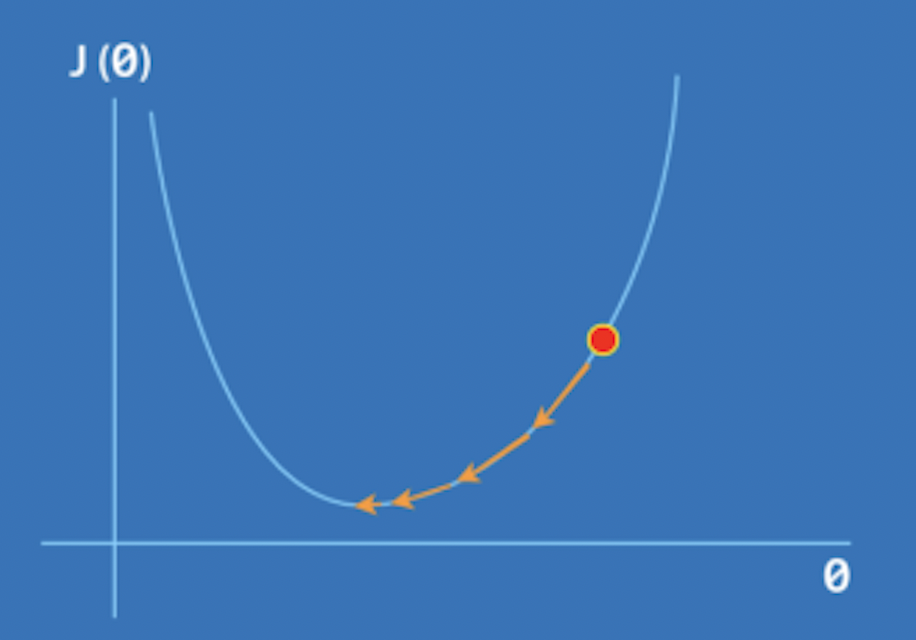
\includegraphics[width=8cm]{images/10.png}
  \centering
\end{figure}

The overall representation of Gradient Descent in linear regression would take on a similar form as given in the plot above, and given that the step size governs the speed and feasibility of convergence, it leads us to inquire about the following matters:

\subsection{What if the step size is too small?}

The plot obtained with very small step size would look something like the plot given below
\begin{figure}[H]
  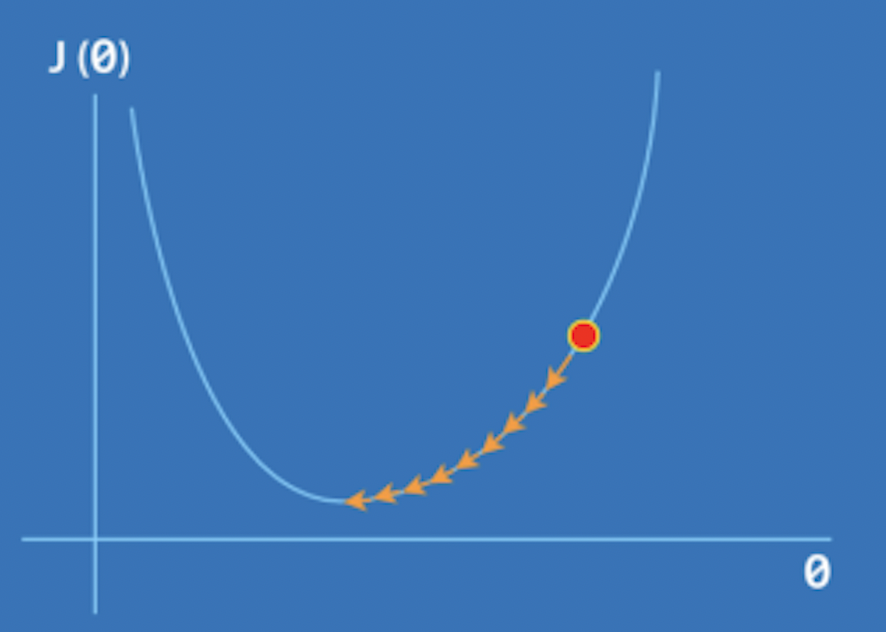
\includegraphics[scale=0.3]{images/11.png}
  \centering
\end{figure}

From the plot, we can conclude that the loss will take very long to converge since we only update by a small value each time. This may also result in never reaching the optimal point if we train using a (fixed) maximum number of epochs.

\subsection{What if the step size is very large?}

The plot obtained with very large step size would look something like the plot given below
\begin{figure}[H]
  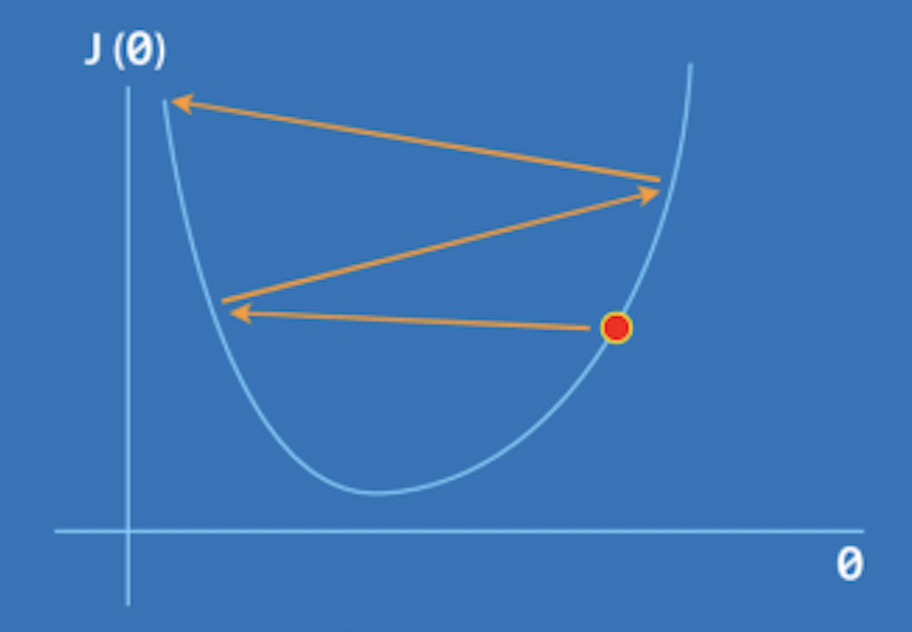
\includegraphics[scale=0.3]{images/12.png}
  \centering
\end{figure}

Clearly in this case the curve will take longer to converge or in the worst case may diverge as seen above.

\section{Weight update rule in GD for linear regression}

The formula for update of $\tc{w}$ is,
\begin{equation}
  \label{eqn:1}
  \tc{w} \leftarrow \tc{w} -\alpha \nabla L(\tc{w})
\end{equation}

\tc{Unregularized Loss}:
\begin{equation}
  L(\tc{w}) = \frac{1}{N}\sum_{i}^N(y_{i} - \tc{w}^{T}\tc{x}_{i})^2
\end{equation}
\begin{equation}
  L(\tc{w}) = \frac{1}{N}\sum_{i}^N(y_{i} - \hat{y_i})^2
\end{equation}
\begin{equation}
  \label{eqn:3}
  \frac{\partial L(\tc{w})}{\partial \tc{w}} = -\frac{2}{N} \sum_{i}^N(y_{i} - \hat{y_{i}})\tc{x}_i = \frac{2}{N} \sum_{i}^N(\hat{y_{i}} - y_{i})\tc{x}_i
\end{equation}

$$\boxed{\tc{w}^{t+1} \leftarrow \tc{w}^{t} - \alpha \frac{2}{N}\sum_{i}^N([\tc{w}^t]^T\tc{x}_i - y_{i})\tc{x}_i}$$

\section{Different Variants of Gradient Descent}
\subsection{(Full) Gradient Descent}

Here, we find the gradient of loss function over the entire training dataset. Our gradient update formula in this case is :
$$
  \tc{w} \leftarrow \tc{w} -\alpha \nabla L(\tc{w}, \D_{train})
$$

The training data can be very large in many applications of ML with millions of data points. Hence, it seems wasteful to compute the full loss function over the entire training set in order to perform only a single parameter update. Hence, we usually use other variations of GD which helps us in avoiding this computationally expensive step of finding gradient of loss over entire data every time.

\subsection{Stochastic Gradient Descent(SGD)}

In this modification of GD, rather than finding gradient of loss over entire training set, we find loss over only single instance of training data that is picked randomly and we update \tc{w} based on the gradient for this loss,
$$\tc{w} \leftarrow \tc{w} - \alpha \nabla L(\tc{w}, \D_{random})$$
where $\D_{random}$ = \{($x_{i}$,$y_{i}$)\}, $(x_{i},y_{i}) \rightarrow$ randomly sampled point in $\D_{train}$\\
Now the issue with this version is that there is a lot of noise in the convergence path of the loss function, as a single data point is not representative of entire data set and this leads to lot of fluctuations in computed gradient. Outliers can lead to training instability in this
case. For example, training may stop prematurely, if for a certain point gradient becomes
zero.

\subsection{Mini Batch Gradient Descent}
In this version of GD, we try to find the best of both the worlds of GD and SGD by using the gradient of loss computed over only a batch (small subset) of original data set. This helps not only in faster gradient calculation but also is less noisier as batch is still a better representative than a single instance used in SGD.
$$
  \tc{w} \leftarrow \tc{w} - \alpha \nabla L(\tc{w}, \D_{batch})
$$

where $\D_{batch}$ = $\{(x_{i},y_{i})\}_{i = 1}^{\mathbb{B}}$, $\mathbb{B} = $batch size\\
Here $\mathbb{B}$ is a hyper parameter. We should know that larger $\mathbb{B}$ is more stable as we approach close to GD and smaller $\mathbb{B}$ is less stable as we move closer to SGD, so the onus lies on us to find that optimal $\mathbb{B}$ that can help us gain the benefit of both the worlds. Also, note that it is a common convention to use $\mathbb{B} = 16,32,64 ...$ usually a power of 2. This method is an improvement over SGD, as it enhances training
stability. Batches are randomly sampled during each epoch.

\section{Probabilistic View of Linear Regression}

For training data $\D = \{(x_{i}, y_{i})\}^{\text{n}}_{i=1}$. Let the target $y_{i}$ have some noise defined as: $$y_{i} = f(x_{i}) + \epsilon_{i}, \qquad \epsilon_{i} \sim \mathcal{N}(0,\sigma^{2})$$
$\epsilon_{i^{'}s}$ are independent and identically distributed (\tc{i.i.d.}), 0 mean Gaussians with the some variance $\sigma^{2}$.(Cov($\epsilon_{i}$, $\epsilon_{j}$) = 0 for all $j \neq i$).
So basically now we can get the following interpretation of data,

\begin{align*}
  \textit{y}_i                               & = f(\textit{x}_i) + \epsilon_i                                                                                                               \\
  \implies \textit{y}_i                      & = \tc{w}^T\textit{x}_i + \epsilon_i                 &                                                                                        \\
  \implies \textit{y}_i                      & \sim \mathcal{N}(\tc{w}^{T}\textit{x}_i , \sigma^2)                                                                                          \\
  \implies \text{P}(y_{i}\mid x_{i}, \tc{w}) & \sim \mathcal{N}(\tc{w}^{T}x_{i} \sigma^{2}),       & \hfill \text{[where }\text{P}(y_{i}\mid x_{i}, \tc{w}) \text{ is likelihood function]}
\end{align*}

For training data $\D = \{(\mathit{x}_{i}, \mathit{y}_{i})\}^{\text{n}}_{i=1}$,
$$
  \text{P}(y_{1}, y_{2}, \ldots, y_{n}\mid x_{1}, x_{2}, \ldots, x_{n}, \tc{w}) = \prod_{i}\text{P}(y_{i}\mid x_{i}, \tc{w})
$$
where $y_{i}$'s are conditionally independent given $x_{i}$'s.

$$
  \implies \log\text{P}(y_{1}, y_{2}, \ldots, y_{n}\mid x_{1}, x_{2}, \ldots, x_{n}, \tc{w}) = \sum_{i}\text{log P}(y_{i} \mid x_{i}, \tc{W})
$$

Note, here we can use log likelihood instead of likelihood because of following reasons,
\begin{itemize}
  \item Does not change the maxima or minima of function as log is monotonic function
  \item Mathematical convenience
  \item Computational convenience as it is easier to add many small values than to multiply them as they might underflow if multiplied
\end{itemize}
\chapter{Probabilistic Model of Linear Regression}
\section{Introduction}

The probabilistic model of linear regression provides a way to understand and interpret linear regression models from a probabilistic view. \\

Consider training data $\D$ :
$$
  \D = \{(\x_i,y_i)\}_{i=1}^n
$$

\tc{Assumption}: The relation between the input features $\x$ and the target $y$ can be represented by a linear equation with some added noise $\epsilon$:
$$
  y_i = \w^T\x_i + \epsilon_i
$$

\tc{Noise}: The noise component $\epsilon$ signifies the fluctuation within the data that contributes towards uncertainty in the target values and cannot be explained by the linear relationship. Assume that it follows a Gaussian distribution with mean 0 and variance $\sigma^2$
$$
  \epsilon_i \sim \mathcal{N}(0, \sigma^2)
$$

In other words, $\epsilon_i$'s are independent and identically distributed (i.i.d.) Gaussian random variables with zero-mean and the same variance $\sigma^2$. Now, we can represent target $y_i$ as a Gaussian distribution with mean $\w^T\x_i$ and variance $\sigma^2$
$$
  y_i \sim \mathcal{N}(\w^T\x_i, \sigma^2)
$$

Given training data $\D = \{(\x_i, y_i)\}_{i=1}^{n}$ where feature vector $\x_i \in \mathbb{R}^{d}$, target $y_i \in \mathbb{R}$,
$$
  P(y_i \mid \x_i, \w)=\frac{1}{\sqrt{2\pi}\sigma} e^{-\frac{(y_i - \w^T\x_i)^2}{2\sigma^2}}
$$
$$
  \text{Likelihood : } \quad P(y_1, y_2, \ldots, y_n \mid \x_1, \x_2, \ldots, \x_n) = \pi_i P(y_i \mid \x_i, \w)
$$
$$
  \text{Log Likelihood : } \quad \log P(y_1, y_2, \ldots, y_n \mid \x_1, \x_2, \ldots, \x_n) = \underset{i}{\sum} \log P(y_i \mid \x_i, \w)
$$

The likelihood function models how well the observed data fits the assumed model. In case of linear regression, it measures the probability of observing the actual target values given the parameter vector w and feature vectors.

\section{Maximum Likelihood Estimation}

The process of finding the best-fitting model often involves estimating the model's parameters in a way that maximizes the likelihood of observing the actual data. This estimation process is known as Maximum Likelihood Estimation (MLE). It is a \textit{Frequentist} view in machine learning. \\

For the model, $y_i$(target value) represented as a Gaussian distribution $\mathcal{N}(\w^T\x_i, \sigma^2)$, the parameter of interest is the weight vector $\w$. We need to find $\w$ that maximizes the likelihood function. Maximizing likelihood function is equivalent to maximizing log likelihood function. (The $\log$ function is strictly increasing, and thus maximizing the log likelihood gives the same solution as maximizing the likelihood function.)
$$
  \w_{\text{MLE}} = \argmax_{\w} \underset{i}\sum \log P(y_i \mid \x_i, \w)
$$

\subsection{Motivating Example}
You want to estimate the probability of a biased coin landing on heads. The probability that the outcome is head for a coin toss is $\theta$.  Let us say your data contains $N$ coin tosses with $N_H$ heads and $N_T$ tails. What is the maximum likelihood estimate of $\theta$ ?\\

Likelihood function: probability of data, given parameter $\theta$
\begin{align*}
  P(D\mid\theta)               & = \theta^N_H(1-\theta)^N_T                                              \\
  \implies \theta_{\text{MLE}} & = \argmax_{\theta} \log P(\D \pipe \theta)                              \\
                               & = \argmax_{\theta} \log \left( \theta^{N_H} (1-\theta)^{N_T} \right)    \\
                               & = \argmax_{\theta} \left( N_H \log \theta + N_T \log (1-\theta) \right)
\end{align*}

To find $\theta_{\text{MLE}}$, we need to find the derivative of $N_H \log \theta + N_T \log (1-\theta)$ w.r.t. $\theta$, set to zero and solve for $\theta$:
\begin{align*}
  \frac{N_H}{\theta_{\text{MLE}}} & - \frac{N_T}{1-\theta_{\text{MLE}}} = 0 \\
  \implies \theta_{\text{MLE}}    & =\frac{N_H}{N_H+N_T}=\frac{N_H}{N}
\end{align*}

\subsection{Question}
Say you have a coin with P $\in$ \{0.4,0.6\} \\
Data: 3 coin tosses; 2 heads, 1 tail \\
What is MLE of P ? \\

\tc{Solution}:
\begin{align*}
  P(D\mid\theta)_{\theta = 0.4} & = (0.4)^2 (0.6)                 \\
  P(D\mid\theta)_{\theta = 0.6} & = (0.6)^2 (0.4)                 \\
  P(D\mid\theta)_{\theta = 0.6} & > P(D\mid\theta)_{\theta = 0.4} \\
  \tc{Answer}                   & = 0.6
\end{align*}

\subsection{MLE for linear regression}
\begin{align*}
  w_{\text{MLE}} & = \argmax \sum_i \log P(y_i \mid \x_i, \w)                                                  \\
                 & = \argmax \sum_i \log ( \mathcal{N}(\w^T\x_i, \sigma^2))                                    \\
                 & = \argmax \sum_i \log \frac{1}{\sqrt{2\pi}\sigma} e^{-\frac{(y_i - \w^T\x_i)^2}{2\sigma^2}} \\
                 & = \argmax C - \sum_i {\frac{(y_i - \w^T\x_i)^2}{2\sigma^2}}                                 \\
  w_{\text{MLE}} & = \argmin \sum_i {(y_i - \w^T\x_i)^2}
\end{align*}

\begin{itemize}
  \item MLE under Gaussian noise distribution is equivalent to the least squares solution.
  \item MLE under Laplacian noise distribution is equivalent to Least Absolute Deviation solution.
  \item A significant drawback of Maximum Likelihood Estimation (MLE) arises when working with limited data, as it can lead to overfitting due to its heavy reliance on the available dataset.
\end{itemize}

\section{Bayesian Parameter Estimation}
In MLE, observations are random variables while parameters are not. On the contrary, in the Bayesian framework, parameters are also treated as random variables alongside observations. Parameters have an underlying \tc{prior distribution} which encode beliefs prior to observing the data. As MLE has a high tendency to overfit, we switch to a different estimation, namely the \tc{Maximum Aposteriori Estimation} with the hope of alleviating overfitting using prior information.

\section{Maximum Aposteriori Estimate ( MAP )}

Maximum A Posteriori (MAP) estimation focuses on incorporation of prior knowledge into estimating the underlying model parameters which are denoted by $\Theta$. We assume a prior distribution $\Pb(\Theta)$ for parameters $\Theta$ (before observing the data $\D$). \\

By Bayes' theorem, we have :
$$
  \Pb(\Theta \pipe \D) = \frac{\Pb(\D \pipe \Theta)\Pb(\Theta)}{\Pb(\D)}
$$

$\bm{\Pb(\Theta \pipe \D)}$ is the \tc{posterior} probability for the model parameters $\Theta$ given data $\D$. \\
$\bm{\Pb(\D \pipe \Theta)}$ is the \tc{likelihood} of observing the data given model parameters \& $\bm{\Pb(\Theta)}$ is the \tc{prior}.
\begin{align*}
  \Theta_{\text{MAP}} & = \arg \max\limits_{\Theta} \Pb(\Theta \pipe \D)                             \\
                      & = \arg \max\limits_{\Theta} ( \log \Pb(\D \pipe \Theta) + \log \Pb(\Theta) )
\end{align*}

\tc{Note:} The posterior is directly proportional to the product of likelihood and the prior functions as shown by the following equation,
\begin{align*}
  \Pb(\Theta \pipe \D) & \propto  \Pb(\D \pipe \Theta)  \Pb(\Theta)           \\
                       & \propto \log \Pb(\D \pipe \Theta) + \log \Pb(\Theta)
\end{align*}

\subsection{Coin example (MAP estimate)}

Suppose, we have a biased coin and N\textsubscript{H} and N\textsubscript{T} are the number of heads and tails obtained.\\ Likelihood ($\Pb\D \pipe \Theta$) , i.e, the probability of data given the parameter $\Theta$ is given by the following equation,
$$
  \Pb(\D \pipe \Theta)=\Theta^{N_H}(1-\Theta)^{N_T}
$$

What is a good prior on $\Theta$ ? \\
\tc{Beta distribution} is a good candidate for prior because the functional form of prior matches with that of the likelihood.
\begin{align*}
  \Beta(\Theta,\alpha,\beta) = c\,\Theta^{\alpha-1}(1-\Theta)^{\beta-1} &  & [c= \frac{\Gamma(\alpha + \beta)}{\Gamma(\alpha)\Gamma(\beta)},\; \Gamma(.) \text{ is the gamma function} ]
\end{align*}

Hence, the posterior will be
\begin{align*}
  \Pb(\Theta,\D) & \propto \Pb(\D \pipe \Theta) \Pb(\Theta)                 \\
                 & \propto c\,\Theta^{N_H+\alpha-1}(1-\Theta)^{N_T+\beta-1} \\
                 & \propto \Beta(\Theta,N_H+\alpha,N_T+\beta)
\end{align*}

\section{Conjugate Priors}
For a likelihood P($\D \pipe \Theta$) coming from a family of distributions $d_{1}$, a prior (from a family $d_{2}$) is said to be a conjugate prior if the posterior distribution also comes from the family $d_{2}$. ($d_{2}$ could also be from the same family as $d_{1}$).

\subsection{Coin example}
Continuing with the coin example mentioned above, the probability of getting N\textsubscript{H} heads and N\textsubscript{T} tails upon tossing a biased coin with the probability of getting head as $\Theta$ (Bernoulli distribution), is given by,
$$
  \Beta(N\textsubscript{H}, N\textsubscript{T}, \Theta) = \Theta^{N\textsubscript{H}}(1-\Theta)^{N\textsubscript{T}}
$$

Also, the PDF for beta distributions is given as,
$$
  \Beta(\Theta, \alpha, \beta) = c.\Theta^{\alpha - 1}(1-\Theta)^{\beta - 1}
$$

The posterior is proportional to the product of likelihood and prior and putting their values we have,
\begin{align*}
  P(\Theta \pipe \D) & \propto  P(\D \pipe \Theta)  P(\Theta)                                                      \\
                     & \propto \Theta^{N\textsubscript{H} + \alpha - 1}(1-\Theta)^{N\textsubscript{T} + \beta - 1} \\
                     & \propto \Beta(\Theta, N\textsubscript{H} + \alpha, N\textsubscript{T} + \beta)
\end{align*}

Hence,
$$
  \Theta_{MAP} = \argmax ((N_H+\alpha-1)\log(\Theta) + (N_T+\beta-1)\log(1-\Theta))
$$

On maximizing it, we get
\begin{align*}
  \frac{N_H+\alpha-1}{\Theta} & - \frac{N_T+\beta-1}{1-\Theta} = 0            \\
  \implies \Theta_{MAP}       & = \frac{N_H+\alpha-1}{N_H+N_T+\alpha+\beta-2}
\end{align*}

Compared to the MLE estimate $\Theta_{\text{MLE}} = \frac{N_H}{N}$, MAP estimate has extra counts denoted by $\alpha$ and $\beta$. \\

We can see that as $N \to \infty \Theta_{\text{MAP}}$ converges to $\Theta_{MLE}$. This represents the fact that prior beliefs become less representative over more data. This is encapsulated in the \href{https://en.wikipedia.org/wiki/Bernstein\%E2\%80\%93von\_Mises\_theorem}{Bernstein - von Mises Theorem}. Further, we also see that in essence, the prior data is enforcing a belief of a ``pre-existing" $\alpha - 1$ heads out of $\alpha + \beta - 2$ tosses. For this reason, these numbers can also be thought of as pseudo coin counts. \\

\tc{Additional Note}: There are a large number of exponential families that serve as conjugate priors for different distributions due to their exponential mathematical form.
\begin{enumerate}
  \item Beta distribution serves as conjugate prior for Bernoulli \& Binomial likelihoods.
  \item Normal distribution is a conjugate prior for itself, i.e. a Gaussian distribution is a conjugate prior for other Gaussian likelihoods, however, inverse gamma distribution also is a conjugate prior for Gaussian likelihood.
  \item Dirichlet prior is used as conjugate for Multinomial distributions.
\end{enumerate}

\subsection{Linear Regression MAP Estimate}

Given the probabilistic setup of Linear Regression, we try to estimate the weights $\w$.

Let's consider zero mean Gaussian Prior on the weights $\w$ with covariance matrix as scaled identity matrix, i.e.
\begin{align*}
  \mathcal{P}\left(\w\right) & = \mathcal{N}\left(0,\frac{\mathbf{I}}{\lambda}\right)                                                                                    \\
                             & = \frac{1}{(2\pi)^{d/2}\sqrt{\det(\mathbf{I}/\lambda)}} \exp{\left(-\frac{1}{2}\w^T\left(\frac{\mathbf{I}}{\lambda}\right)^{-1}\w\right)} \\
                             & = \left(\frac{\lambda}{2\pi}\right)^{d/2} \exp{\left(-\frac{\lambda}{2}\w^T\w\right)}                                                     \\
                             & = \left(\frac{\lambda}{2\pi}\right)^{d/2} \exp{\left(-\frac{\lambda}{2}\norm{\w}_2^2\right)}
\end{align*}

Now, if we try to find the MAP estimate for $\w$,
\begin{align*}
  \w_{\text{MAP}} & = \underset{\w}{\arg\max}
  \bigl(\mathcal{P}\left( \D \, | \, \w\right) \, \mathcal{P}\left(\w\right)\bigr) \\
                  & =\underset{\w}{\arg\max}
  \Bigl(\log\bigl(\mathcal{P}\left( \D \, | \, \w\right)\bigr) + \log\bigl(\mathcal{P}\left(\w\right)\bigr)\Bigr)
\end{align*}

Using the MLE equation to rewrite the log-likelihood term and plugging in the prior term gives us,
\begin{align*}
  \w_{\text{MAP}} & = \underset{\w}{\arg\max}
  \left(\frac{-1}{2\sigma^2} \sum_{i=1}^n \left(y_i - \w^T\x_i\right)^2 + \frac{d}{2}\log\left(\frac{\lambda}{2\pi}\right) - \frac{\lambda}{2}\norm{\w}_2^2\right) \\
                  & = \underset{\w}{\arg\min}
  \left(\frac{1}{2\sigma^2} \sum_{i=1}^n \left(y_i - \w^T\x_i\right)^2 + \frac{\lambda}{2}\norm{\w}_2^2\right)
\end{align*}

Recall that this is same as the $L_2$-regularised linear regression (or Ridge Regression).\\

\tc{NOTE}: By changing the prior, we can get various types of regularisations. For example, using a Laplace Prior will give \(L_1\) Regularisation (or Lasso Regression)

\section{Bias and Variance of Estimates}
Natural question that arises after creating different types of Linear Regression models is that "How do we evaluate whether the predictor is good or not?". \\

One of the metric that we use to generate the model is Training Loss, but this does not tell whether the model will be able to generalize or not. Hence, to define whether a model is good or not, we look at the Test Loss. \\

So, we try to decompose the Expected Test Loss and it turns out that it has 3 components
\begin{enumerate}
  \itemsep-0.3em
  \item Variance
  \item Bias
  \item Noise (or Irrecoverable error/ Unavoidable error)
\end{enumerate}

Out of these, Variance and Bias are inherent to the model and Noise is inherent to the data (due to inaccuracies in measurements).

\subsection{Bias}

Let us assume that we are sampling data from a true distribution
$$
  y = f(\x) + \epsilon
$$

where $\epsilon$ is a zero mean Gaussian Noise with standard deviation $\sigma$. Let $h_{\w}(.)$ be the predictor for a given data $\D$. Then the bias of the given model for a particular $\x$ can be defined as follows
$$
  \text{Bias} = \mathbb{E}\left[h_\w(\x)\right] - f(\x)
$$

Note that the expectation is over various choice of training data set $\D$ which will give rise to various $h_\w(.)$. Also, $\x$ is fixed value and the expectation does not depend on it.
To explain the meaning of bias, let us sample multiple different data sets from the given true distribution and find the predictor function for each of them. Then the bias represents how close the average of these predictor functions is to the true distribution.

\begin{figure}[H]
  \centerline{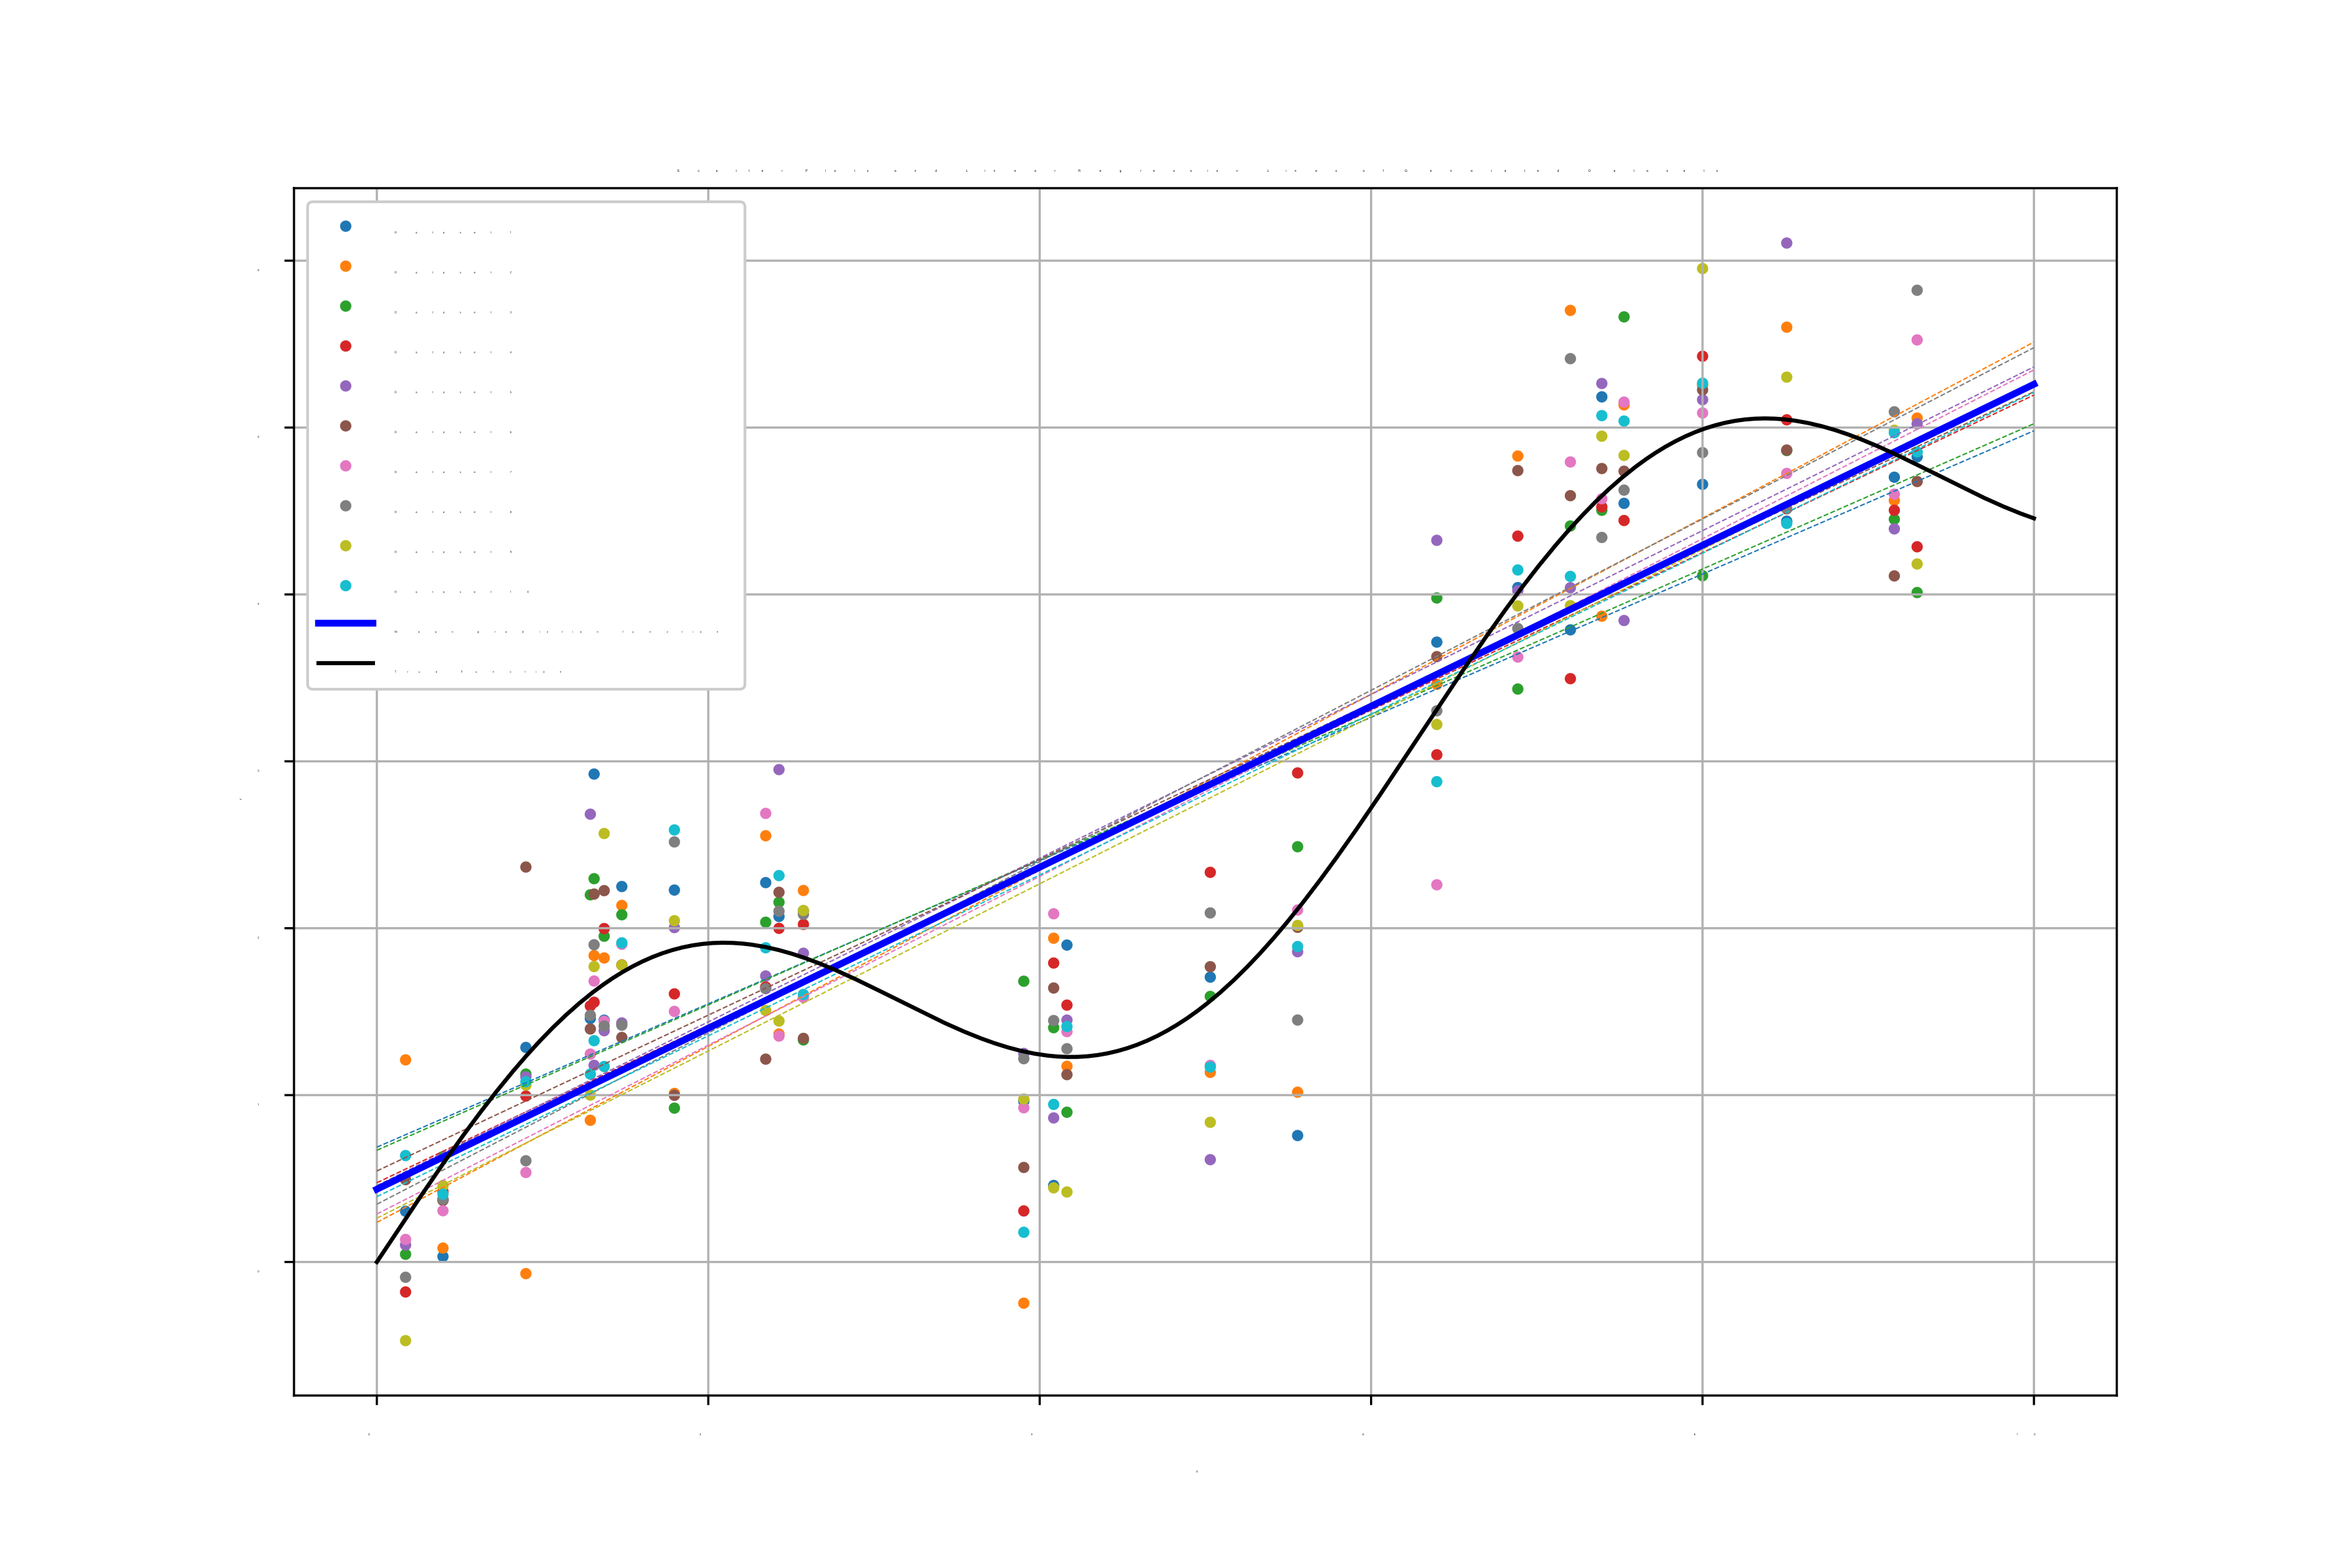
\includegraphics[width = 0.7\textwidth]{images/13.png}}
  \caption{Showing various regression arising from various data-sets and the mean of them}
  \label{fig}
\end{figure}

\subsection{Variance}

Considering the same setup as before, the variance of the given model for a particular \(\x\) can be defined as follows
\begin{equation}
  \text{Variance} = \mathbb{E}\left[\bigl(h_\w(\x)-\mathbb{E}\left[h_\w(\x)\right]\bigr)^2\right]
\end{equation}
Note that the expectation is over various choices of training data set \( \D\) which will give rise to various \(h_\w(.)\). Intuitively, variance of given model is basically the variance of different predictor functions that we get by varying the data set \( \D\). Qualitatively, it measures the spread of predictor functions in figure \ref{fig}.

\subsection{Noise}

Noise is the unavoidable error in the data caused by the errors in measurement. The expression for this error is as follows
\begin{equation}
  \text{Noise} = \mathbb{E}\left[\bigl(y-f(\x)\bigr)^2\right]
\end{equation}
Note that this expectation is over the random noise (i.e. $\epsilon$ in this case) and not dependent on the data set. This reduces to
\begin{align*}
  \text{Noise} & = \mathbb{E}\left[(\epsilon)^2\right] \\
               & = \text{Var}(\epsilon)                \\
               & = \sigma^2
\end{align*}

\subsection{Analysing Unregularized Linear Regression}

Let us assume that we have the same model as before, i.e.
$$
  y = f(\x) + \epsilon \;\;\text{and}\;\; \epsilon \sim \mathcal{N}(0,\sigma^2)
$$

As mentioned before, we are trying to find the expected test error. Let us denote the test data point as $(\widetilde{\x},\widetilde{y})$ i.e. $\widetilde{y} = f(\widetilde{\x}) + \widetilde{\epsilon}$. Then we have to find
$$
  E_{\text{test error}} = \mathbb{E}_{\widetilde{\epsilon},\D}\left[\bigl(\widetilde{y} -h_\w\left(\widetilde{\x}\right)\bigr)^2\right]
$$

\tc{NOTE}: Here, we are assuming that $\xt$ is a constant while taking the expectation, i.e. LHS should ideally be parameterized as $E_\text{test error}(\xt)$. This would also mean that $\yt$ (which is a random variable) is only dependent on $\widetilde{\epsilon}$.
\begin{align*}
  E_{\text{test error}} & = \mathbb{E}\left[\bigl(\widetilde{y} -h\left(\widetilde{\x}\right)\bigr)^2\right]                                                                \\
                        & = \expe{\yt^2} + \expe{\hxt^2} - 2 \, \expe{\yt} \, \expe{\hxt}                                                                                   \\
                        & = \expe{\bigl(\yt - \expe{\yt}\bigr)^2} + \expe{\yt}^2 + \expe{\bigl(\hxt - \expe{\hxt}\bigr)^2} + \expe{\hxt}^2 - 2 \, \expe{\yt} \, \expe{\hxt} \\
                        & = \expe{\bigl(\yt - f(\xt)\bigr)^2} + \expe{\bigl(\hxt - \expe{\hxt}\bigr)^2} + \expe{\hxt}^2  + \expe{\yt}^2 - 2 \, \expe{\yt} \, \expe{\hxt}    \\
                        & = \expe{\bigl(\yt - f(\xt)\bigr)^2} + \expe{\bigl(\hxt - \expe{\hxt}\bigr)^2} + \Bigl(\expe{\hxt}  - \expe{\yt}\Bigr)^2                           \\
                        & = \expe{\bigl(\yt - f(\xt)\bigr)^2} + \expe{\bigl(\hxt - \expe{\hxt}\bigr)^2} + \Bigl(\expe{\hxt}  - f(\xt)\Bigr)^2                               \\
                        & = \text{Noise} + \text{Variance} + \text{Bias}^2
\end{align*}

\begin{mdframed}
  \tc{Explanations of steps}:
  \begin{itemize}
    \item The predicted value $h(\xt)$ depends only on the data set and hence it is independent of the actual value $\yt$ (which is only dependent on $\widetilde{\epsilon}$)
    \item Using the definition of variance we can get $\expe{Y^2} = \expe{\bigl(Y-\expe{Y}\bigr)^2} + \expe{Y}^2$
    \item Also, note that $\expe{\yt} = \expe{f(\xt)+\widetilde{\epsilon}} = \expe{f(\xt)}+\expe{\widetilde{\epsilon}} = f(\xt)$ as the noise is zero mean and $\xt$ is a constant (as mentioned before)
  \end{itemize}
\end{mdframed}

\pagebreak
\subsection{Variance-Bias Trade-Off}

Let us look at the use of the above-mentioned formula. \\

Consider the following case where we have used a very high complexity model for linear regression.

\begin{figure}[H]
  \centering
  \begin{subfigure}{.4\textwidth}
    \centering
    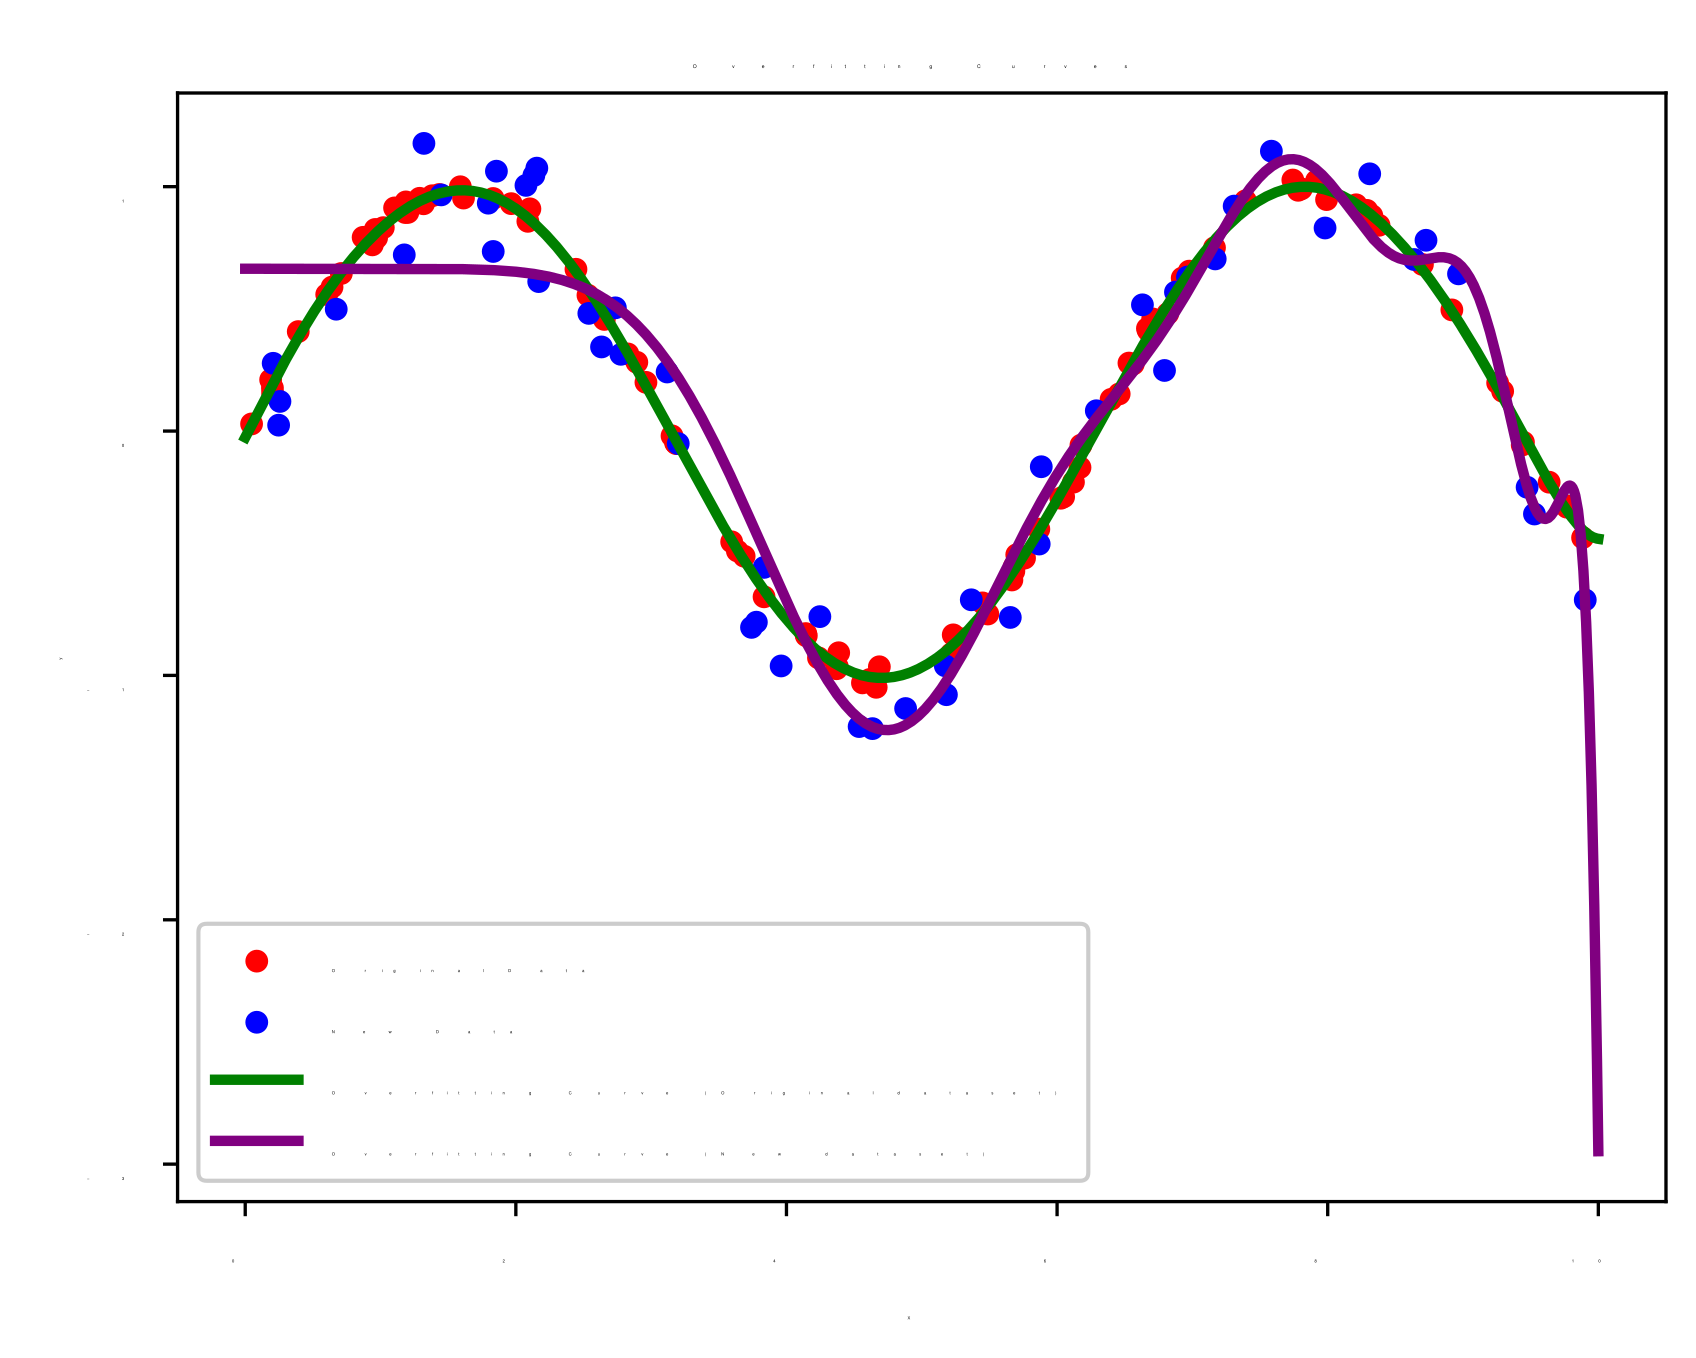
\includegraphics[width=\linewidth]{images/14.png}
    \caption{Over-fitting - High Variance, Low Bias}
  \end{subfigure}%
  \begin{subfigure}{.4\textwidth}
    \centering
    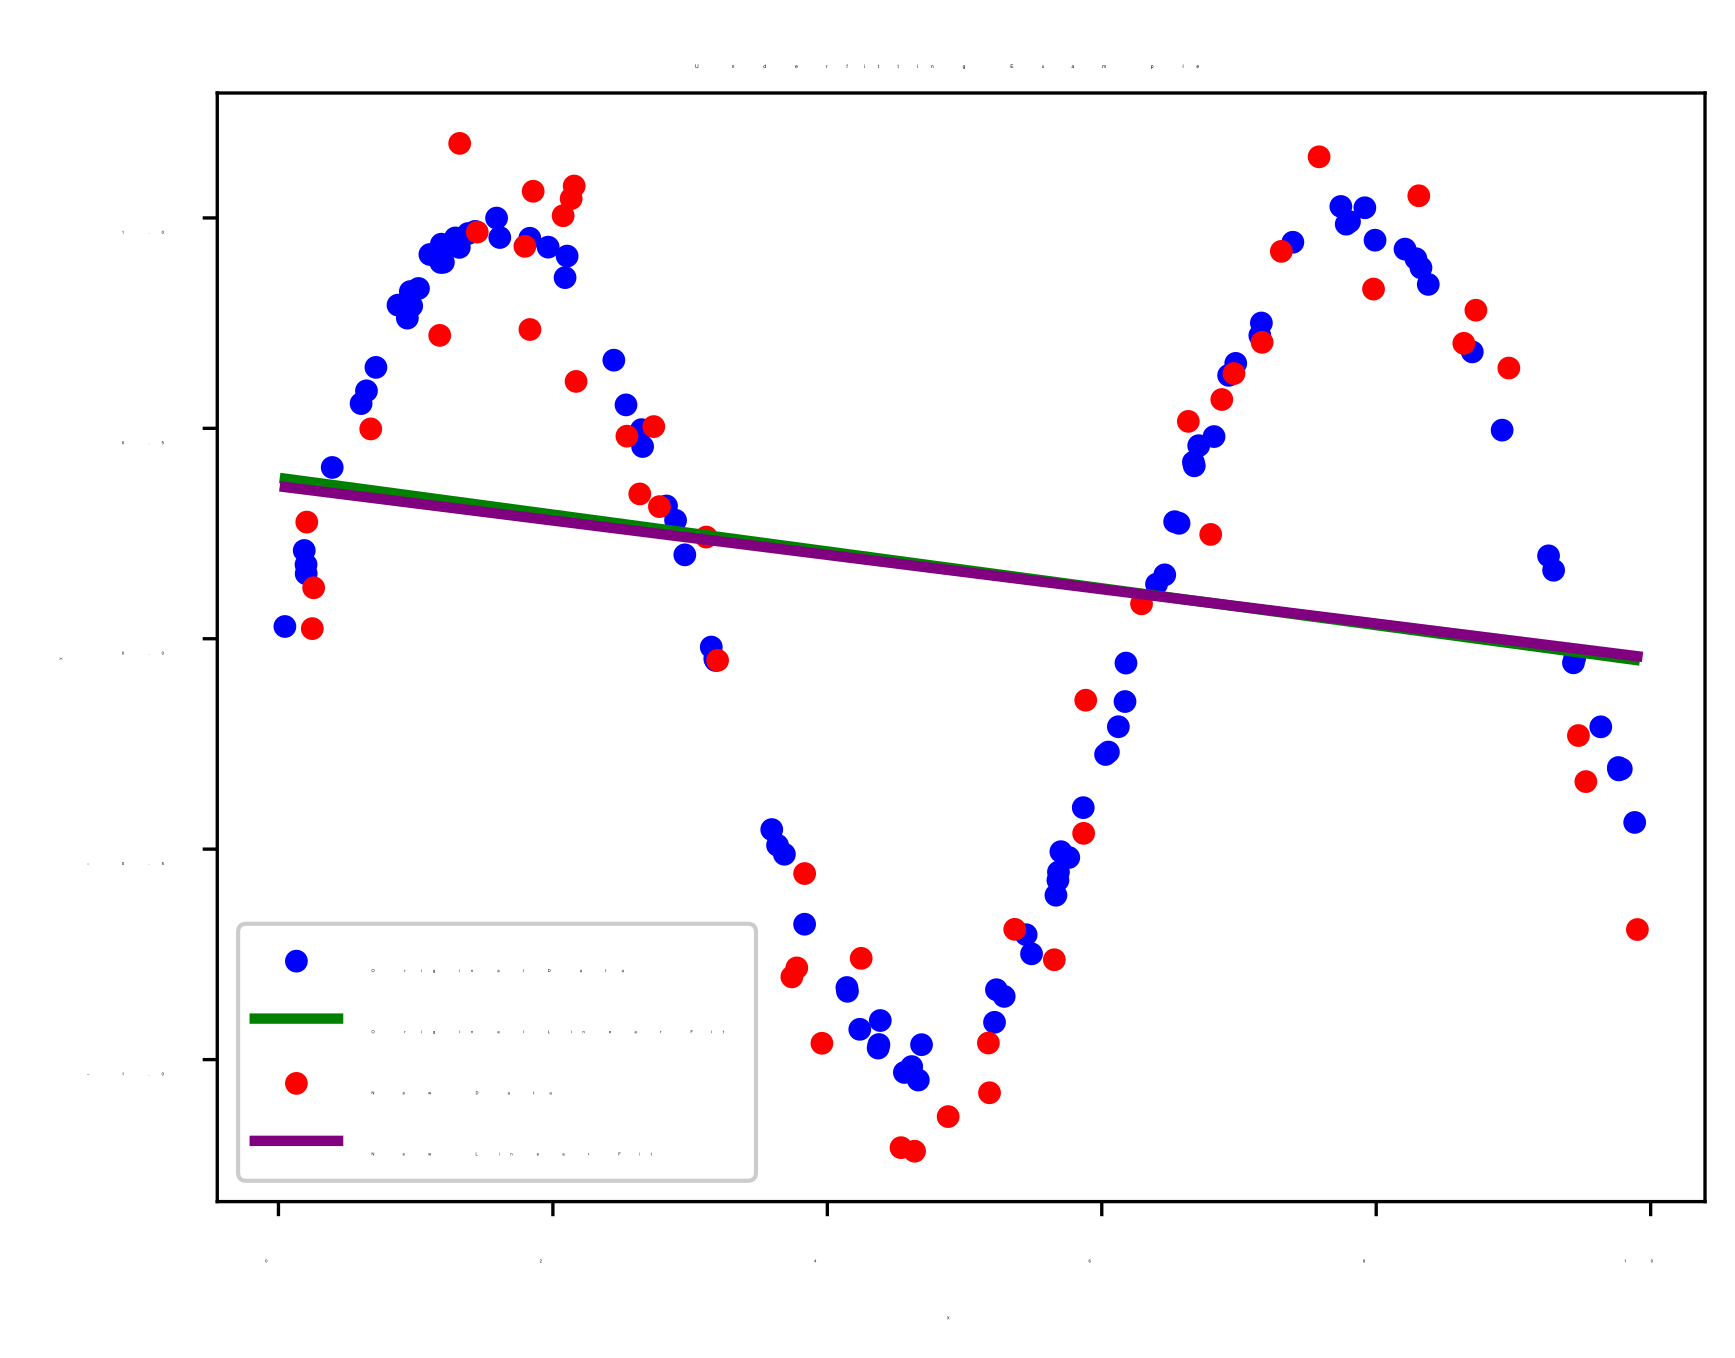
\includegraphics[width=\linewidth]{images/15.png}
    \caption{Under-fitting - Low Variance, High Bias}
  \end{subfigure}
  \caption{Analysing models using bias and variance}
\end{figure}

It is evident that the bias of this high-complexity model is very low. But, as we change the dataset slightly, we can see that there is too much variation in the newly fitted curve. This means that this high-complexity model also has high variance. Similarly, we can consider a low-complexity model such as linear. Here, the predicted values deviate significantly from the actual function, and hence the bias is high. But, changing the dataset has very less effect on the predictor function, suggesting that there is low variance. \\

The ideal model is one that strikes a balance between bias and variance. Highly complex models, like high-order polynomials, may overfit, resulting in \tc{low bias but high variance}. In contrast, lower complexity models might not capture all data complexities, leading to \tc{high bias and low variance}. Both can yield high test errors.

\begin{figure}[H]
  \centering
  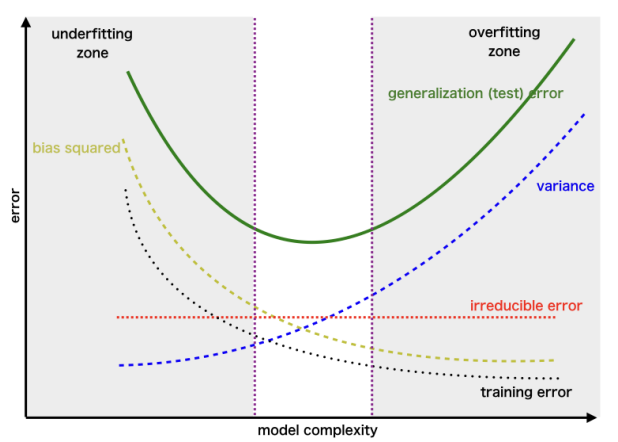
\includegraphics[width = 0.4\textwidth]{images/16.png}
  \caption{Variance Bias Trade-off with Expected Test Error/Generalisation Error}
\end{figure}

Hence, there is an inherent trade-off between variance and bias. We can't make both of them arbitrarily small at the same time. \\

\begin{mdframed}
  Recall $L_2$-Regularised model where,
  $
    \w_{\text{ridge}} = \underset{\w}{\arg\min}
    \left(\norm{y - \mathbf{X}\w}_2^2 + \lambda\norm{\w}_2^2\right)
  $
  . As $\lambda$ increases, the loss penalises high variation of $\w$ and hence the variance decreases. However, this is also reducing the flexibility of model and hence leading to increased bias.
\end{mdframed}


\chapter{Logistic Regression}
\section{Introduction}

Logistic regression involves a classification task, we instead of predicting a real value, we try to predict the label class for each input.

A natural way to re-purpose linear regression for classification tasks is to predict the class label as follows:
$$
  \hat{y} = \begin{cases}
    1 \ \text{if} \ \tc{w}^T \tc{x} \geq \tau \\
    0 \ \text{otherwise}
  \end{cases}
$$

where $\tau$ acts as the threshold, and is a hyper-parameter for the model.

However, this approach has certain limitations:

\begin{itemize}
  \item It is not easy to pick a good value for $\tau$.
  \item It is difficult to calibrate the prediction quality, that is estimating the confidence the model has for a certain prediction.
\end{itemize}

To overcome these issues, we modify the range of score that the model assigns from $(-\infty, \infty)$ to $(0, 1)$ which can then be interpreted as the ``probability'' of the input $\tc{x}$ being in class $\hat{y} = 1$.

\section{Logistic Regression}

\subsection{Sigmoid Function}

The first task is to collapse the score from $(\infty, \infty)$ to $(0, 1)$. To do so, we use the \tc{Sigmoid Function}, which is as follows:

\begin{equation*}
  \boxed{\sigma(x) = \frac{1}{1 + \exp(-x)}}
\end{equation*}

Observe that sigmoid is a monotonically increasing function with the range being $(0, 1)$. Another property which makes it useful for our task is the form it's derivative takes:

\begin{align*}
  \sigma'(x) & = \frac{-1}{(1 + e^{-x})^2} \cdot (-e^{-x})            \\
             & = \frac{1}{1 + e^{-x}} \cdot \frac{e^{-x}}{1 + e^{-x}} \\
             & = \sigma(x)\cdot(1 - \sigma(x))
\end{align*}

The derivative of the sigmoid function can hence be written in terms of the sigmoid function itself, a property we will use later.

\subsection{Model}

The model used in logistic regression outputs the probability of the input vector $\tc{x}$ having class label $y = 1$ as follows:
\begin{align*}
  P(y = 1 \pipe \tc{x}, \tc{w})           & = \sigma(\tc{w}^T \tc{x})                              \\
  P(y = 0 \pipe \tc{x}, \tc{w}) = 1 - P(y & = 1 \pipe \tc{x}, \tc{w}) = 1 - \sigma(\tc{w}^T\tc{x})
\end{align*}

\begin{center}
  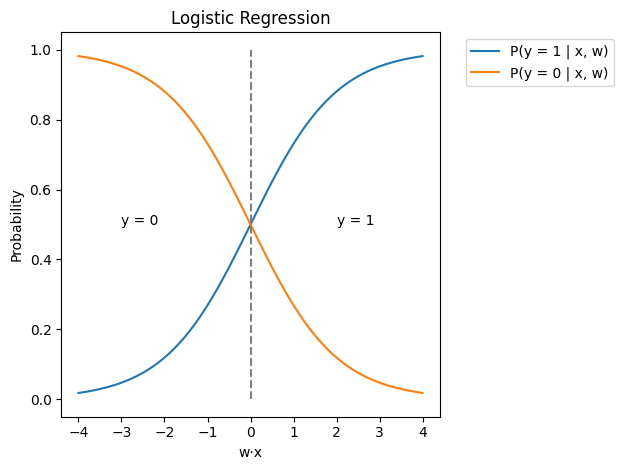
\includegraphics[scale=0.35]{images/05_01.png}
\end{center}

We then predict the label $\hat{y}$ as the label which has higher probability. Hence $\hat{y} = 1$ if:

\begin{align*}
           & \frac{P(y = 1 \pipe \tc{x}, \tc{w})}{P(y = 0 \pipe \tc{x}, \tc{w})} > 1 \\
  \implies & \frac{\sigma(\tc{w}^T\tc{x})}{1 - \sigma(\tc{w}^T\tc{x})} > 1           \\
  \implies & \exp(\tc{w}^T\tc{x}) > 1                                                \\
  \implies & \tc{w}^T\tc{x} > 0
\end{align*}

Hence, the \tc{hyperplane} $\tc{w}^T \tc{x} = 0$ acts as a \tc{decision boundary} in the sense that all input vectors $\tc{x}$ lying ``above'' the boundary (that is $\tc{w}^T \tc{x} > 0$) are given label $1$ and rest are given label $0$.

\begin{center}
  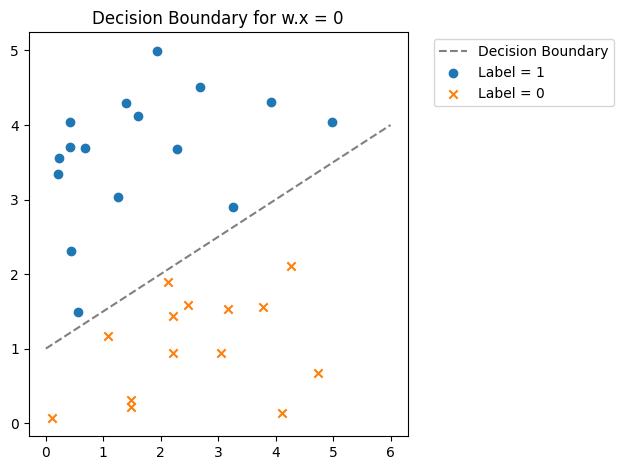
\includegraphics[scale=0.4]{images/05_02.png}
\end{center}

Observe that logistic regression yields a linear decision boundary. Hence it can perfectly classify the training points for \tc{linearly separable data}. \\

\fbox{
  \begin{minipage}{\textwidth}
    \tc{Linearly Separable Data}: A data-set $ \D$ is linearly separable if $\exists \tc{w}$ such that $\forall$ positive training points ($y = 1$), $\tc{w}^T\tc{x} > 0$ and $\forall$ negative training points ($y = 0$), $\tc{w}^T\tc{x} < 0$.
  \end{minipage}
} \\

This puts a severe restriction on the data-sets which can be classified using logistic regression. Consider a simple example, where $\tc{x} = [x_1, x_2]^T \in \mathbb{R}^2$ :

\begin{equation*}
  y = \begin{cases}
    1 \qq{if} x_1 \cdot x_2 > 0 \\
    0 \qq{otherwise}
  \end{cases}
\end{equation*}

\begin{center}
  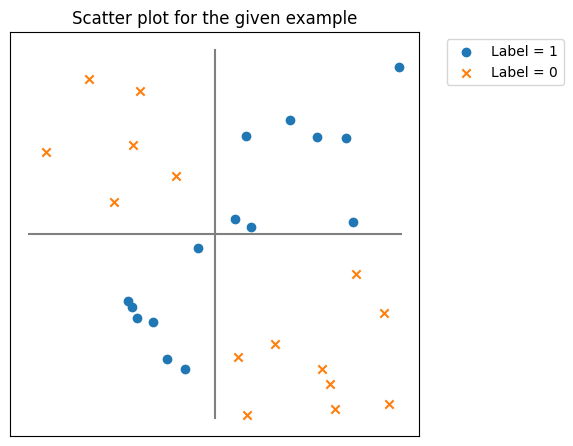
\includegraphics[scale=0.35]{images/05_03.png}
\end{center}

Observe that a Logistic Regression Classifier will not be able to find a good linear decision boundary for the above data. However, adding a feature to get $\phi(\tc{x}) = [1, x_1, x_2, x_1 x_2]^T$ makes the data linearly separable and enables the model to find a perfect weight vector $\tc{w} = [0, 0, 0, 1]^T$ to classify the data.

Hence, to get better results, we may have to add new features to the input vector before training the model.

\subsection{Parameter Estimation}

Since the output of model is a probability distribution on the labels, it is natural to estimate the parameters $\tc{w}$ as the \tc{Maximum Likelihood Estimate} for the observed data (training data-set). Hence,

\begin{align*}
  \tc{w}^* & = \underset{\tc{w}}{\text{argmax}} \prod_{i=1}^{| \D_{\text{train}}|} P(y_i | \tc{x}_i, \tc{w})                                           \\
           & = \underset{\tc{w}}{\text{argmax}} \sum_{i=1}^{| \D_{\text{train}}|} \log P(y_i | \tc{x}_i, \tc{w}) \qq{(Maximum Conditional Likelihood)} \\
           & = \underset{\tc{w}}{\text{argmin}}  \sum_{i=1}^{| \D_{\text{train}}|} -\log P(y_i | \tc{x}_i, \tc{w}) \qq{(Corresponding Loss Function)}
\end{align*}

Here, $ P(y_i \pipe \tc{x}_i, \tc{w}) $ is shorthand for $ P(\hat y_i = y_i\pipe \tc{x}_i, \tc{w}) $, where $P(\hat y_i = 1 \pipe \tc{x}_i, \tc{w}) = \sigma(\tc{w}^T \tc{x}_i)$.

Hence, the loss associated with a single data point is:

\begin{align*}
  L_{\tc{w}} (\tc{x}_i, y_i) = \begin{cases}
                                 -\log P(y_i = 1 \pipe \tc{x}_i, \tc{w}) \qq{if} y_i = 1 \\
                                 -\log (1 - P(y_i = 1 \pipe \tc{x}_i, \tc{w})) \qq{if} y_i = 0
                               \end{cases}
\end{align*}

Combining them,

\begin{equation*}
  \boxed{L (\tc{w}, \tc{x}_i, y_i) = -y_i \log P(y_i = 1 \pipe \tc{x}_i, \tc{w}) - (1 - y_i) \log (1 - P(y_i = 1 \pipe \tc{x}_i, \tc{w}))}
\end{equation*}

Total loss across the dataset then would be,

\begin{equation*}
  L  (\tc{w},  \D) = \sum_{i = 1}^{| \D|} \underbrace{-y_i \log P(y_i = 1 \pipe \tc{x}_i, \tc{w}) - (1 - y_i) \log (1 - P(y_i = 1 \pipe \tc{x}_i, \tc{w})) }_{\text{(Binary) Cross Entropy Loss}}
\end{equation*}

This loss is called the binary cross entropy loss because of the similar structure as the formula for cross-entropy loss in information theory. Some properties about the above defined cross entropy loss:

\begin{itemize}
  \item It is a convex loss function
  \item It is differentiable
  \item There is no closed form solution for the optimal parameter $\tc{w}^*$. Hence techniques such as gradient descent are used to optimise the model.
\end{itemize}

To calculate the gradient, note that \begin{align*}
  \nabla_{\tc{w}} \sigma(\tc{w}^T \tc{x}_i) & =  \sigma(\tc{w}^T \tc{x}_i)(1-\sigma(\tc{w}^T \tc{x}_i))\nabla_{\tc{w}} \tc{w}^T \tc{x}_i \\ &= \sigma(\tc{w}^T \tc{x}_i)(1-\sigma(\tc{w}^T \tc{x}_i))\tc{x}_i
\end{align*}
$$
  \implies \nabla_{\tc{w}} \log \sigma(\tc{w}^T \tc{x}_i) = (1-\sigma(\tc{w}^T \tc{x}_i))\tc{x}_i
$$
$$
  \nabla_{\tc{w}} \log (1 - \sigma(\tc{w}^T \tc{x}_i)) = -\sigma(\tc{w}^T \tc{x}_i)\tc{x}_i
$$
\begin{align*}
  \implies \nabla_{\tc{w}}L  (\tc{w},  \D) & =  \sum_{i = 1}^{| \D|}-y_i  (1-\sigma(\tc{w}^T \tc{x}_i))\tc{x}_i + (1 - y_i) \sigma(\tc{w}^T \tc{x}_i)\tc{x}_i \\&= \sum_{i = 1}^{| \D|}(\sigma(\tc{w}^T\tc{x}_i)-y_i) \tc{x}_i\\
                                           & = \sum_{i = 1}^{| \D|}(\hat y_i-y_i) \tc{x}_i
\end{align*}

The form of the gradient is very similar to that in linear regression, with $\hat y = \sigma(\tc{w}^T\tc{x}_i)$

This also shows convexity, since
\begin{align*}
  \nabla^2_{\tc{w}}L  (\tc{w},  \D) & = \nabla_{\tc{w}} \cdot \nabla_{\tc{w}} L (\tc{w},  \D)                                         \\
                                    & = \sum_{i = 1}^{|\D|} \nabla_{\tc{w}} \cdot (\sigma(\tc{w}^T\tc{x}_i)-y_i) \tc{x}_i             \\
                                    & = \sum_{i = 1}^{|\D|} \sigma(\tc{w}^T \tc{x}_i)(1-\sigma(\tc{w}^T \tc{x}_i)) \ ||\tc{x}_i||_2^2 \\
                                    & > 0
\end{align*}

and hence, gradient descent would be good option to minimise loss and find optimal paramters.

\section{Logistic Regression with Regularization}

Logistic regression is capable of perfectly classifying linearly separable data. But there may be mulitple weight vectors that can separate the data. Let us consider the case in which the dataset is linearly separable and the true decision boundary is represented by straight lines.

\begin{center}
  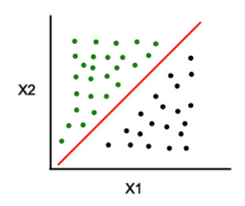
\includegraphics[scale=0.8]{images/05_04.png}
\end{center}

For the data given in the above diagram, the true decision boundary is represented by the straight line $x_1 - 2x_2 = 0$. However, the problem with the supposed values of $w_1 = 1, w_2 = -2$ is that they can be scaled up arbitrarily because the constant term is $0$. Hence, it raises the question as to what are the values of $\tc{w}$ that the logistic regression classifier is likely to converge at ? \\

We know that
$$
  \Pb(y_i = 1 \pipe \tc{x}_i, \tc{w}) = \sigma(\tc{w}^\top \tc{x}) = \frac{1}{1+\exp(-\tc{w}^\top \tc{x})}
$$

The aim of the classifier is to maximise the above probability for the points in the training dataset and thus it is likely that it will pump up the values of the weights to decrease the value of $\exp(-\tc{w}^Tw\tc{x})$ and thus increasing the value of $\Pb(y_i = 1 \pipe x_i,w)$ to about $1$ for all of the positive samples. Thus, in short it is likely that our classifier would choose high values of the weights $w$. \\

\tc{But is this ideal?}

\begin{center}
  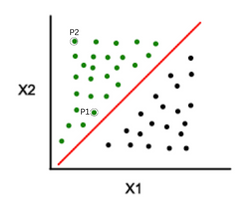
\includegraphics[scale=0.8]{images/05_05.png}
\end{center}

Consider two positive sample points as shown in the above figure, one very close to the decision boundary $P1$, and the other further away from the decision boundary $P2$. We would ideally want a higher value of
$$
  P(y_i = 1 \pipe \tc{x}_i,\tc{w}) = \sigma(\tc{w}^\top \tc{x}) = \frac{1}{1+\exp(-\tc{w}^\top\tc{x})}
$$

for $P2$ than $P1$ as it is far away from the decision boundary and thus confidence of prediction should be higher for this point than $P1$. Ideally, we want data points far from the decision boundary like $P2$ to have a higher probability of being correctly classified by the classifier, while data points near the decision boundary like $P1$ should not be excessively influenced and receive artificially higher probabilities of being classified into one of the regions. But when the values of the coefficients $w$ in logistic regression are arbitrarily high, it diminishes the distinction between data points located near the decision boundary and those far from it as the probability for all the positive samples nearly tends to 1. This occurs because the exponential term in the logistic function causes the probabilities assigned to both types of points to become substantially higher.  \\

To address this issue, we introduce a \tc{regularization term} along with the loss function.
$$
  \tc{w}^*_R = \arg\min_{\tc{w}} \ L_{CE}(\tc{w}, \D) + \lambda||\tc{w}||^2_2
$$

The regularization term's purpose is to impose constraints on the values of $\tc{w}$, preventing them from becoming arbitrarily high. By applying regularization, we effectively limit the coefficients' magnitudes, which helps maintain the proper distinction between data points and prevents the model from assigning overly confident probabilities to points near the decision boundary. \\

The regularization penalty term forces the model to find a balance between minimizing the cross entropy loss (fitting the data) and minimizing the regularization term (keeping coefficients small). This means that the model's predictions are less sensitive to minor fluctuations or noise in the training data. Consequently, the above model becomes more robust and less likely to overfit, leading to a \tc{reduction in variance}. \\

In logistic regression, when the decision boundary is linear, it is relatively straightforward to interpret the model. The feature interpretability of logistic regression models with linear decision boundaries is high which means we can easily assess the importance and relevance of each feature or attribute in making predictions. However, when dealing with non-linear decision boundaries, especially in models with numerous features, interpreting the model and selecting the most informative features becomes much more challenging. \\

There are 2 desired features of classification models:
\begin{enumerate}
  \item The ability to learn complex decision boundaries.
  \item Interpretability of the model i.e. how useful are each of the features/attributes.
\end{enumerate}

Non-linear logistic regression models aren't easily interpretable and so now, we move onto another kind of classifiers which are Decision Tree Classifiers.

\section{Decision Trees: Learning complex decision boundary}
Decision tree is an interpretable model whose final prediction can be written as a \tc{disjunction of conjunctions} based on the attribute values over training instances.

\begin{center}
  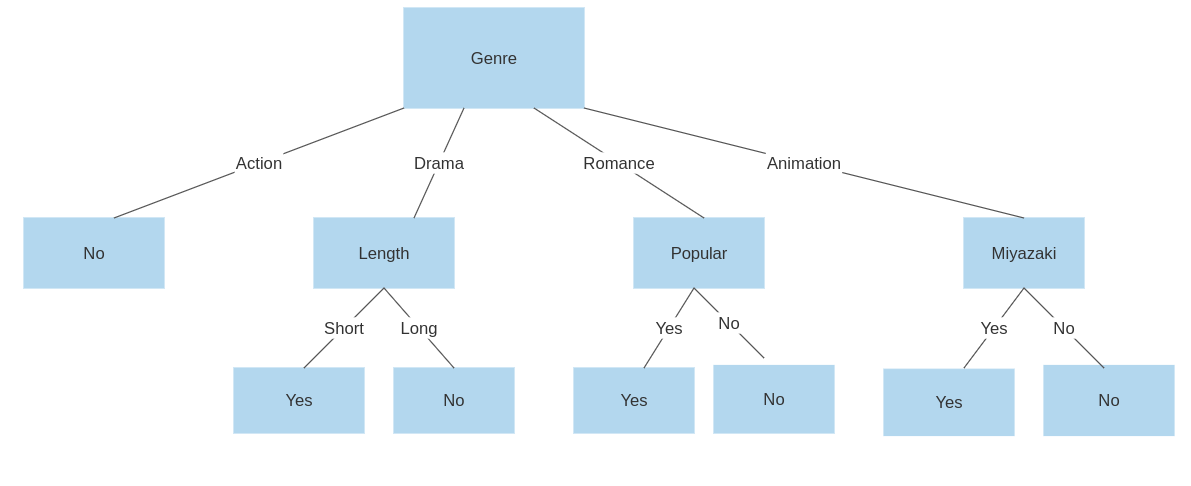
\includegraphics[width=\textwidth]{images/05_06.png}
\end{center}

The above figure is an example of a decision tree. It represets how decisions might be made by a decision tree to classify movies that are liked (represented by 'Yes') or disliked (represented by 'No') by a person. Each node of the tree represents an attribute and each path of the tree represents a conjuction of attributes and the final decision is a disjunction of these conjuctions. For instance for the above tree, the final prediction of the model can be written as
\begin{align*}
   & (Genre = Drama \ \wedge \ Length = Short) \vee (Genre = Romance \ \wedge \ Popular = Yes) \\
   & \vee (Genre = Animation \ \wedge \ Mizayaki = Yes)
\end{align*}

The above expression evaluates to true (yields the value 1) for a 'Yes' instance and evaluates to false (yields the value 0) for a 'No' instance.

\subsection{Decision Boundaries of Decision Trees}
Consider the following xor-like classified dataset

\begin{center}
  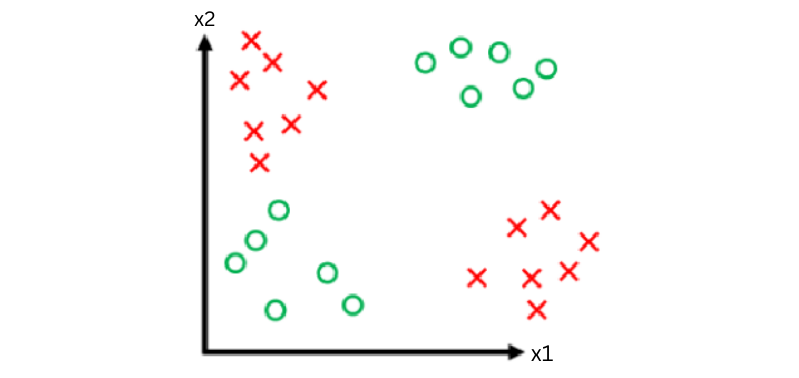
\includegraphics[width=0.8\textwidth]{images/05_07.png}
\end{center}

The x and y axis correspond to 2 attributes of the dataset, $x1$ and $x2$ respectively. The datapoints marked by green circles and the datapoints marked by red crosses represent 2 different categories $(y_{labels})$ say category 1 and category 2 respectively. \\

The following might be the decision tree for the classification of the above dataset.
\begin{center}
  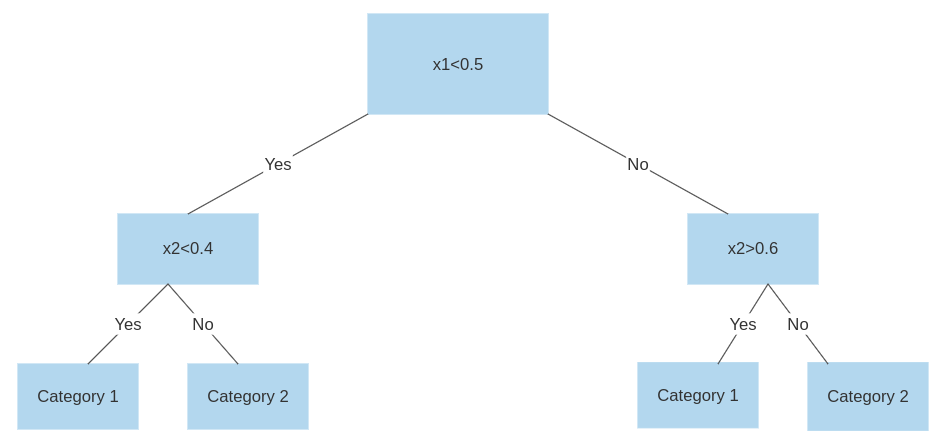
\includegraphics[width=\textwidth]{images/05_08.png}
\end{center}

If the condition in the topmost decision node of the decision tree that is $x_{1} < 0.5$ evaluates to true, we move along the left edge of the tree and right otherwise. After traversing an edge, we either land on the condition(node) $x_{2} < 0.4$ or $x_{2} > 0.6$ respectively. If the condition in the node evaluates to true, we move along the left edge and we move along the right edge in case the condition evaluates to false. If we have moved along the left edge, in this example decision tree, we predict category 1(represented by green circles) or else we predict category 2(represented by red crosses) \\

Thus, on the basis of the above decision tree, the decision boundaries of the decision tree are as follows:
\begin{center}
  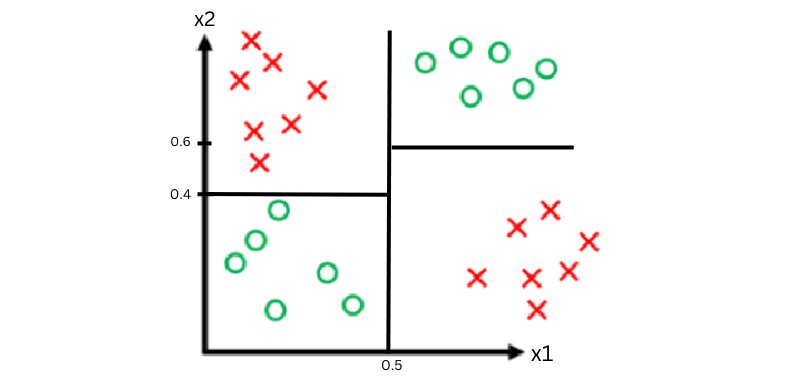
\includegraphics[width=0.8\textwidth]{images/05_09.png}
\end{center}

The vertical line represents the topmost decision node of the decision tree that is $x_{1} < 0.5$ and the two horizontal lines represent $x_{2} < 0.4$ and $x_{2} > 0.6$ respectively. We can see that the decision boundaries are just the depiction of the nodes (the attributes based on which decisions were taken) of the decision tree when plotted on a graph. \\

Thus, as seen above if nodes of the decision tree depend on a single attribute only, then decision trees divide the feature space into \tc{hyper-rectangles} or equivalently we can say that the resulting decision boundaries are axis-parallel hyper-planes.

\begin{mdframed}
  \tc{NOTE}: Instead of axis-parallel hyperplanes, we can even have linear hyper-planes. In the later case, instead of the decision nodes being a linear function of a single attribute, they can be a linear function of 2 or more attributes, say for instance $x_{1} + x_{2}>0$. Thus, in such cases instead of axis-parrallel decision boundaries, we would have locally-linear decision boundaries.
  Typically, axis-parallel hyperplanes are used for decision tree modelling.
\end{mdframed}

\subsection{Finding the optimal Decision Tree}
Unlike the case for logistic regression, finding the smallest Decision Tree that is optimal with respect to some metric (like cross entropy loss etc.) involving all of the attributes is an \tc{NP-hard problem}.

Decision tree estimation is done rather largely \tc{greedily} in which the tree is built recursively.

\vspace{2 mm}

Here's a simple decision tree template:
\begin{itemize}
  \setlength\itemsep{0pt}
  \item Start from an empty node with all instances.
  \item Pick the \tc{best} attribute to split on. For instance in figure 1, genre was chosen as the first attribute
  \item Repeat step 2 recursively for each new node until a \tc{stopping criterion} is met
\end{itemize}
\vspace{2mm}

Now, two important questions arise:
\begin{itemize}
  \setlength\itemsep{0pt}
  \item What is the notion of best attribute and how do we find it?
  \item What is a good stopping criterion?
\end{itemize}
\vspace{2mm}

It is to be noted that a lot of heuristics are involved in decision tree construction which is different from logistic regression we have studied in which we had a clearly formulated optimisation problem and a final solution to the optimisation problem. \\

We will start by reflecting on how to choose the best attribute.

\subsection{Choosing node attributes}

\begin{center}
  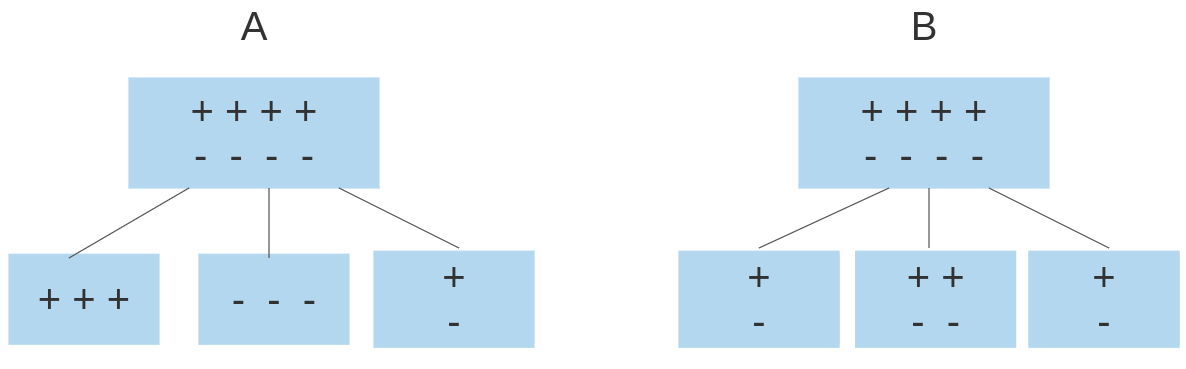
\includegraphics[width=\textwidth]{images/05_10.png}
\end{center}

Unlike the previous trees we have seen, the nodes of the above tree represent the datapoints that would reach these nodes based on the values of some attribute. In both of the above images, the topmost node represents the entire dataset (as no division of the dataset on the basis of some attribute has been done yet). Then on the basis of some attribute which is clearly different for $A$ and $B$, the dataset is divided into 3 datasets which are present in the three child nodes of each parent. \\

Seeing the above classification, it seems intuitive that the attribute on which decision has been taken in $A$ is better than the one in $B$. This is because, $A$'s attribute is leading to nodes that are already largely \tc{homogeneous} and thus the attribute in $A$ immediately effectively reduces the length of the decision tree. \\

On extending the tree, $B$ might later on have better accuracy but the top attribute is just overly building out the tree which is not preferable as overly large trees might lead to overfitting. Thus, our goal somewhat broadly is find simple models that generate good subtrees that get added on and we want the size of subtrees to be as small as possible. \\

\begin{mdframed}
  \tc{Intuition for a good split (attribute)}: A good split for an attribute results in subsets that are (mostly) entirely homogeneous that is the dataset in each split is (mostly) all of the same category.
\end{mdframed}

Now, we need a quantitative way to suit our intuitions for a good attribute and thus we introduce the following concepts.

\subsection{Entropy}

Entropy of a random variable is a measure of \tc{uncertainty} in the value of that random variable. Let $X$ be a random variable and $x$ represent a particular value of the random variable. Entropy  of X is H(X) where H(X) is defined as
$$
  H(X) =  -\sum_{x} \Pb(X=x)\log_{2} (\Pb(X=x))
$$

To understand what $H(X)$ signifies, let's pick up our familiar coin toss example in which the random variable can take the value 1 or 0 on the basis of the result of the coin toss (heads or tails respectively). $H(X)$ for this random variable is plotted below:

\begin{figure}[H]
  \centering
  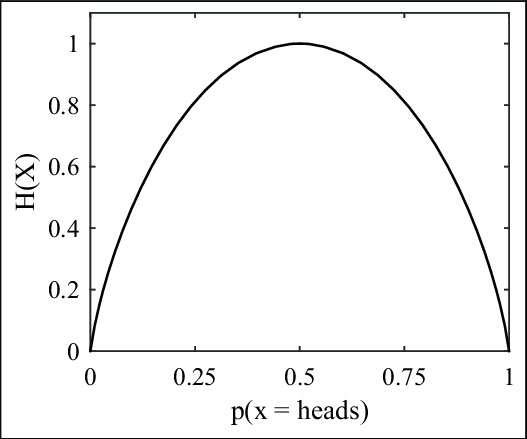
\includegraphics[width=0.4\textwidth]{images/05_11.png}
  \caption{Entropy of a coin toss}
\end{figure}

If the coin is fair (P(Head) = P(Tail) = 0.5) then there is maximum uncertainty in  toss outcome and thus entropy has a maxima at this point and if the coin is heavily biased (e.g P(Head)= 0.9, P(Tail)= 0.1) then there is some certainty about whether it would be head or tail and thus entropy is low. Thus, higher the uncertainty in the outcome of the random variable, higher is the entropy.
Thus it can be said that,
\begin{itemize}
  \item A high value of entropy asserts a nearly uniform distribution . We do not know the next outcome(e.g coin toss).
  \item A lower value of Entropy asserts that the distribution of the random variable has well-defined modes and thus there is some certainty in the outcome of the random variable.
\end{itemize}

\subsection{Entropy of a Dataset}

Entropy of a dataset measures the uncertainty in the group of observations. Consider a dataset $S$ with k classes/labels. Entropy of the dataset $S$ is $H(S)$ where $H(S)$ is defined as
$$
  H(S) =  -\sum_{i=1}^{k} \Pb_{i,S}\log (\Pb_{i,S})
$$

where $\Pb_{i,S}$ is the relative count of instances in $S$ with label i (the probability of randomly selecting an example of class i in $S$).\\
What happens when all instances belong to the same class? $\Pb_{i,s}$ is 1 which implies that entropy of the dataset is 0.

\subsection{Splitting Criterion: Information Gain}

We are building towards deciding on how to choose the best attributes to build our decision tree such that when the data is split on their basis, we achieve maximum possible homogeneity in other words the maximum drop in the entropy within two tree levels. \\

\tc{Information gain}, is simply the reduction in entropy caused by partitioning the dataset $S$ according to a particular attribute.
It determines the quality of splitting and helps to determine the order of attributes in the nodes of a decision tree. \\

Gain of a dataset $S$ for a attribute $a$ is defined as
$$
  Gain(S,a) =  H(S) -\sum_{v \in V(a)}\frac{|S_v|}{|S|} H(s_v)
$$

where $H(S)$ is the entropy of the dataset before spliting on the basis of the attribute $a$, $S_v$ is the subset of dataset $S$ whose instances all have the attribute $a$ taking the value $v$, and thus the term subtracted from $H(S)$ is nothing but the weighted sum of the entropies of the dataset into which the dataset $S$ is split on the basis of attribute $a$. \\

Thus for each node of the decision tree, we find the attribute with the maximum information gain and split on its basis in our decision tree.

\end{document}
